\chapter{مسیریابی برای اجماع ربات‌ها}
%%%%%%%%%%%%%%%%%%%%%%%%%%%%%%%%%%%%%%%%%%%
\section{مقدمه}
در این قسمت به پیاده‌سازی الگوریتم‌های فصل \ref{ch path planning} برای اجماع ربات‌ها به صورت آنلاین پرداخته می‌شود. منظور از آنلاین بودن برنامه‌ریزی این است که در هر گام زمانی، ربات مجددا الگوریتم مسیریابی را اجرا نماید. برای مسیریابی با میدان پتانسیل، در ابتدا اجماع با شکل‌دهی ثابت برای عبور از موانع تلاش می‌کند اما پس از اشاره به ایرادات این روش، در ادامه کار شکل‌گیری پلتون شکسته و دوباره به شکل‌گیری تلاش خواهند کرد. همچنین موانع به صورت ثابت و متحرک خواهند بود.

\section{میدان پتانسیل}
در این قسمت تمامی مسیریابی‌ها تنها با میدان پتانسیل انجام شده است. در ابتدا شکل‌گیری ثابت و سپس شکل‌گیری با قابلیت شکسته شدن مورد بررسی قرار خواهد گرفت. قابل ذکر است که در هر دو روش تا جای ممکن محاسبات به صورت نامتمرکز\LTRfootnote{distributed} بوده است.

\subsection{جلوگیری از برخورد با موانع با شکل‌گیری ثابت}
در این قسمت یک شکل‌گیری ثابت برای دسته ربات‌ها در نظر گرفته شده است. ایده اصلی این است که نیروی جاذبه برای رهبر که در مرکز دسته پلتون حضور دارد و نیروی دافعه برای هر ربات محاسبه گردد و در نهایت نیروی کلی به دست آید. در این راستا برای محاسبه دو ایده برای پیاده‌سازی به وجود می‌آید اول اینکه همانند شکل \ref{Fig platoon-potential-field-simulink} به صورت متمرکز تمام داده‌ها به محاسبه‌گری که مسئول محاسبه مسیر ربات رهبر است فرستاده شود و نیروهای دافعه و جاذبه در آن محاسبه گردند.
\begin{figure}[!h]
	\centering
	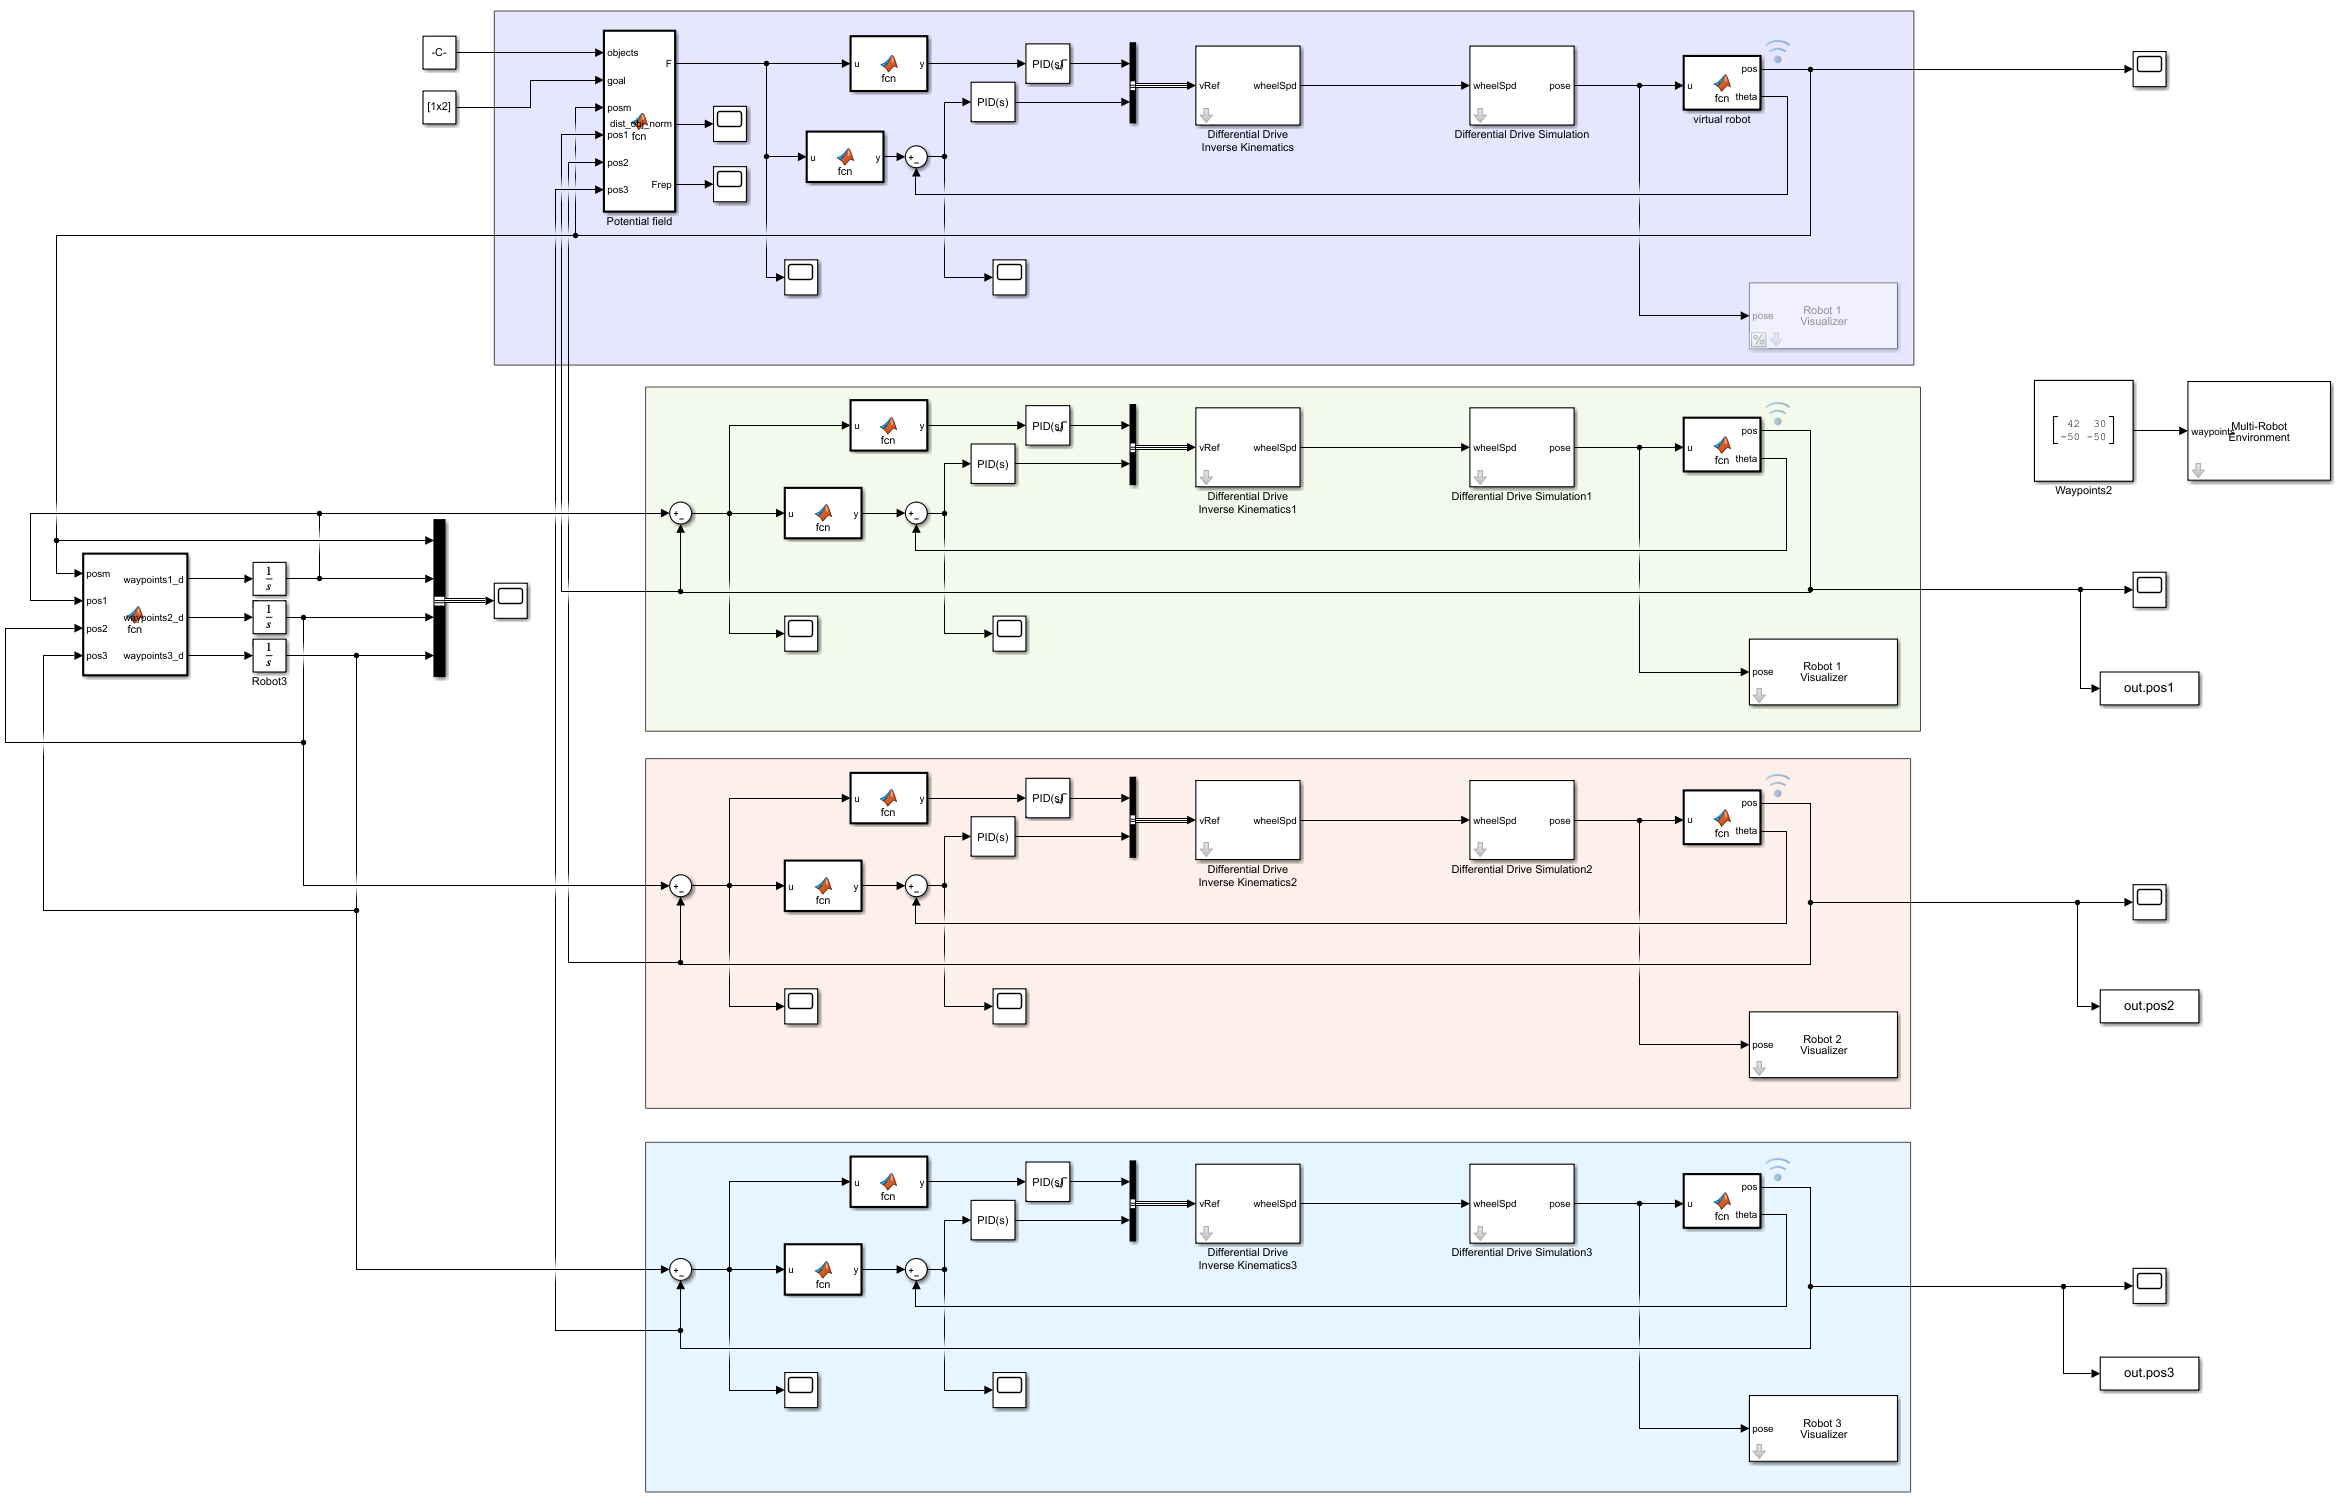
\includegraphics[scale=0.25]{Images/platoon-potential-field-simulink.png}
	\caption{بلوک‌های شبیه‌سازی در روش شکل‌گیری ثابت با محاسبات متمرکز}\label{Fig platoon-potential-field-simulink}
\end{figure}


مکان ربات‌ها برای روش متمرکز به رنگ‌های سبز، آبی و قرمز و موانع با رنگ سیاه در شکل \ref{Fig platoon-potential-field-pos} به نمایش در آمده است.
\begin{figure}[!h]
	\centering
	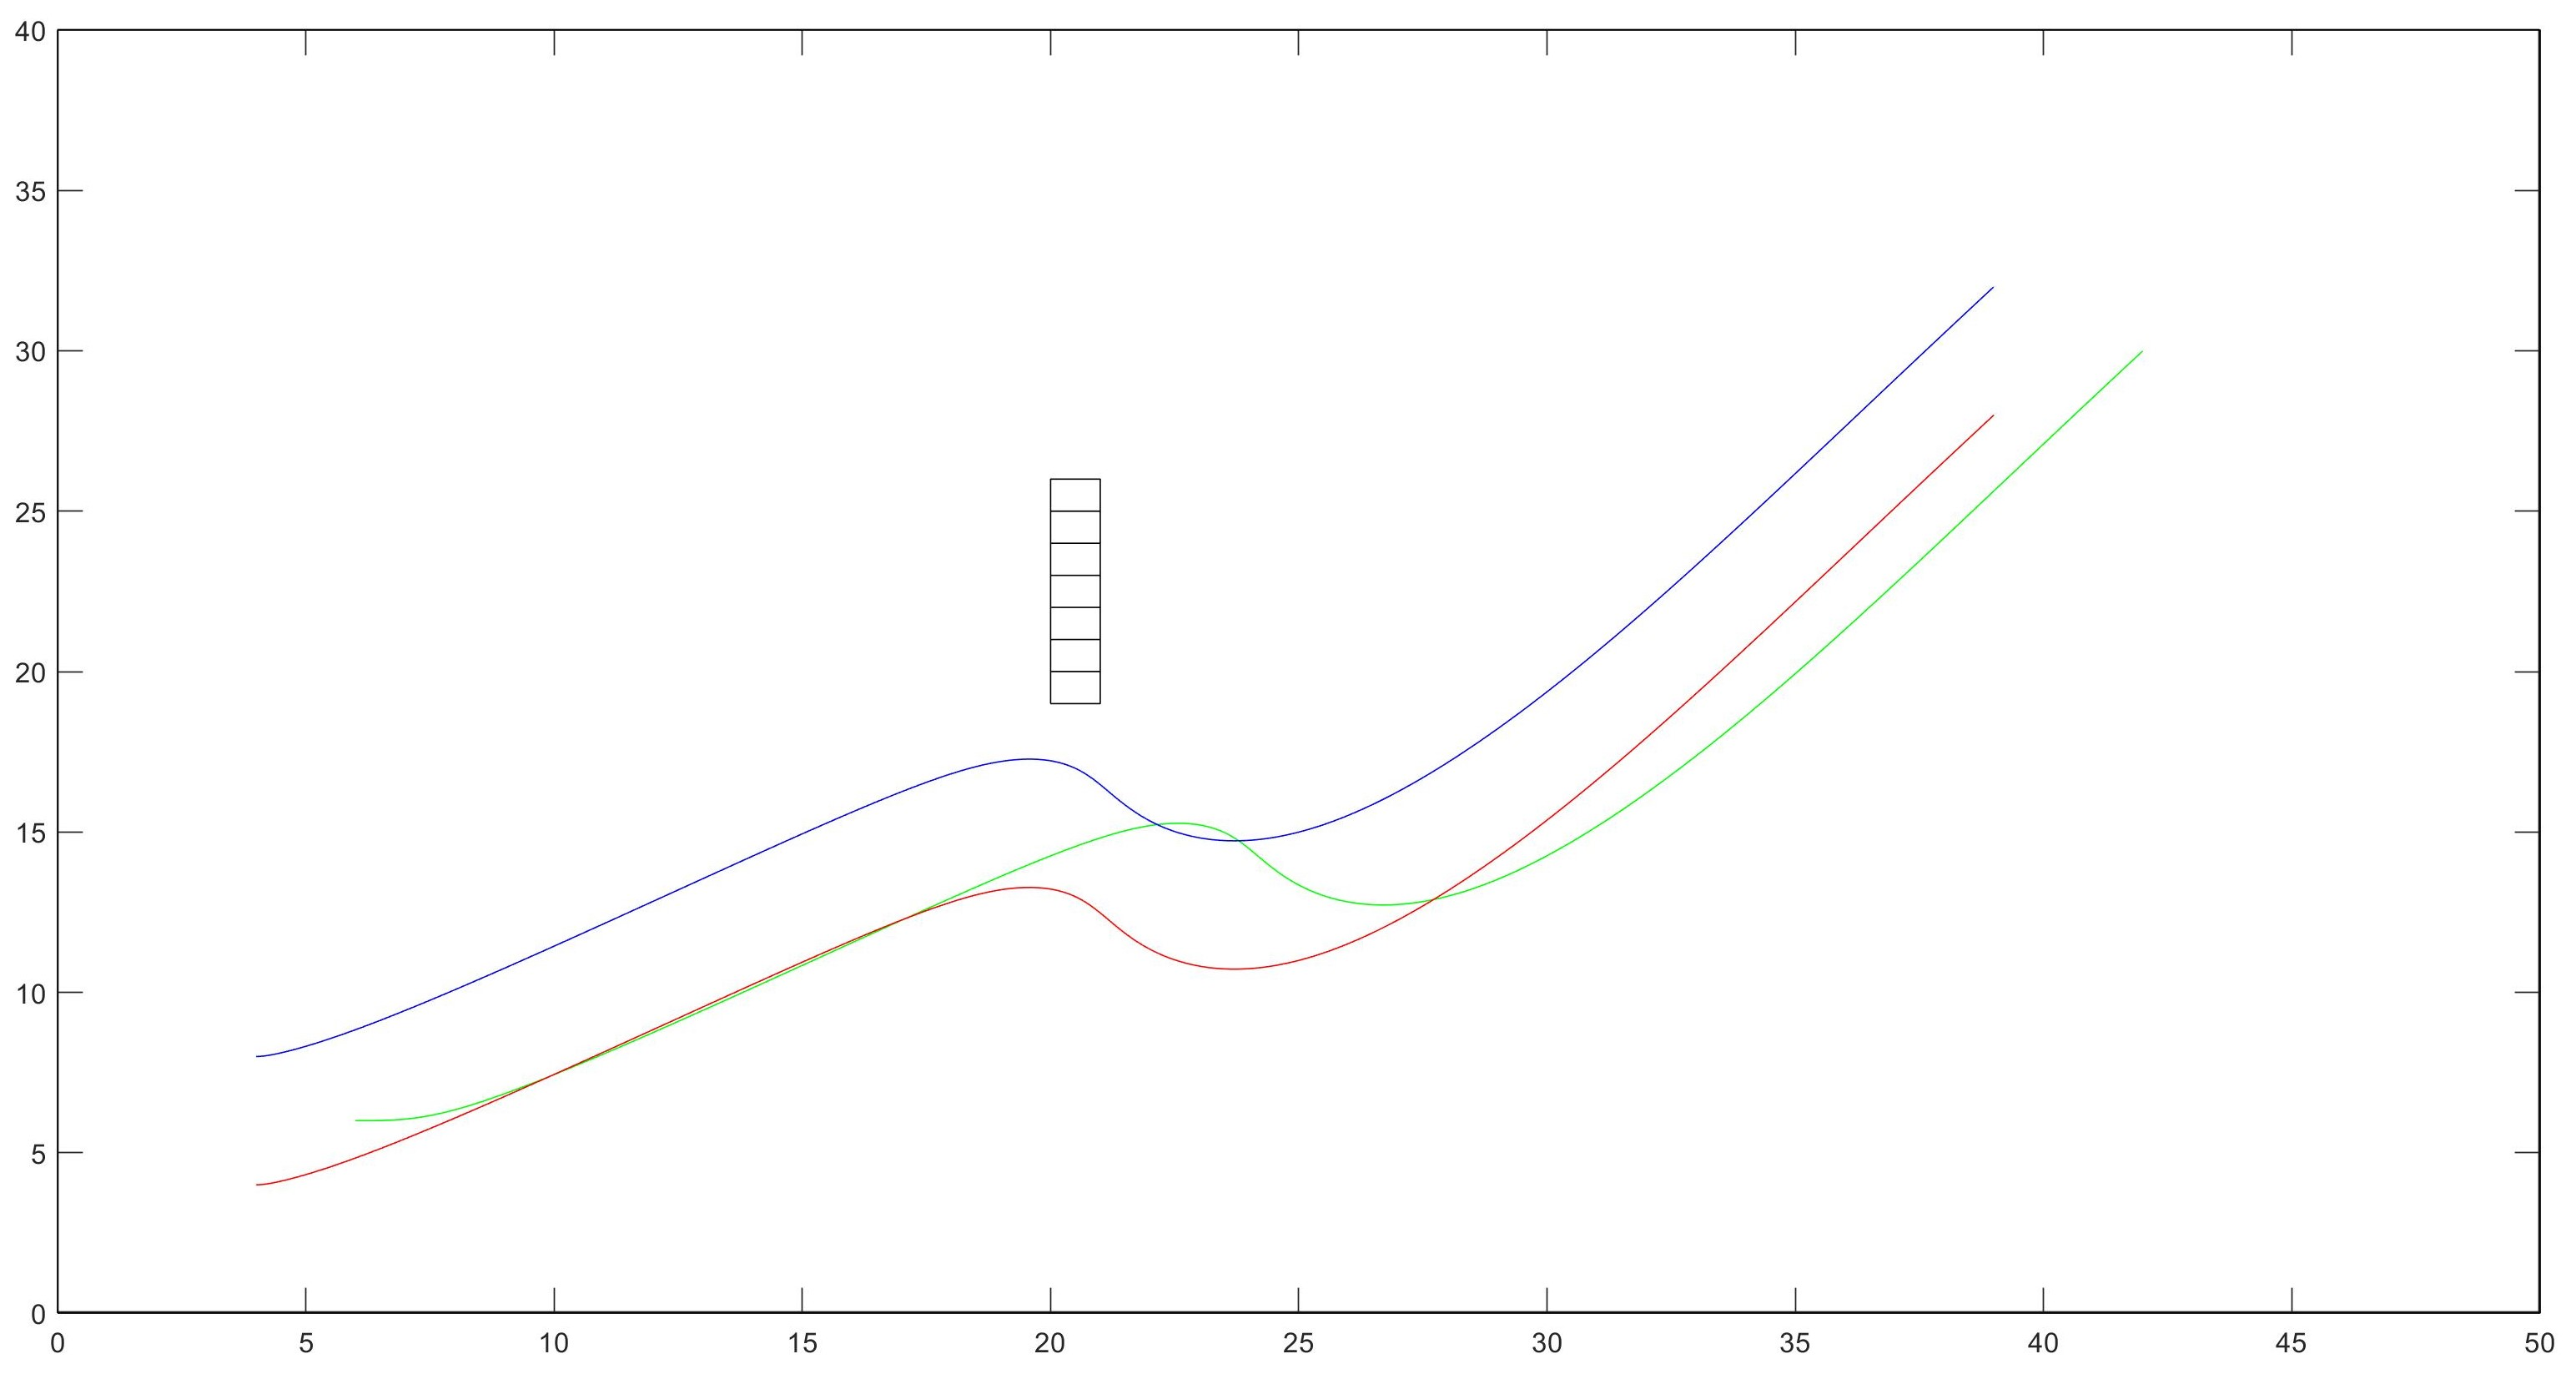
\includegraphics[scale=0.2]{Images/platoon-potential-field-pos.jpg}
	\caption{مکان ربات‌ها در روش شکل‌گیری ثابت با محاسبات متمرکز}\label{Fig platoon-potential-field-pos}
\end{figure}

در روش دوم، برای اینکه دوره محاسبات کاهش یابد، همانند شکل \ref{Fig platoon-potential-field-distributed-simulink} محاسبه نیروی دافعه ناشی از هر ربات، به صورت نامتمرکز و جداگانه در هر ربات محاسبه می‌شود و سپس به ربات رهبر فرستاده می‌شود. محاسبه‌گر ربات رهبر تنها مقادیر را با هم جمع می‌نماید تا به نیروی دافعه برسد. اما نیروی جاذبه همچنان توسط رهبر محاسبه می‌گردد.
\begin{figure}[!h]
	\centering
	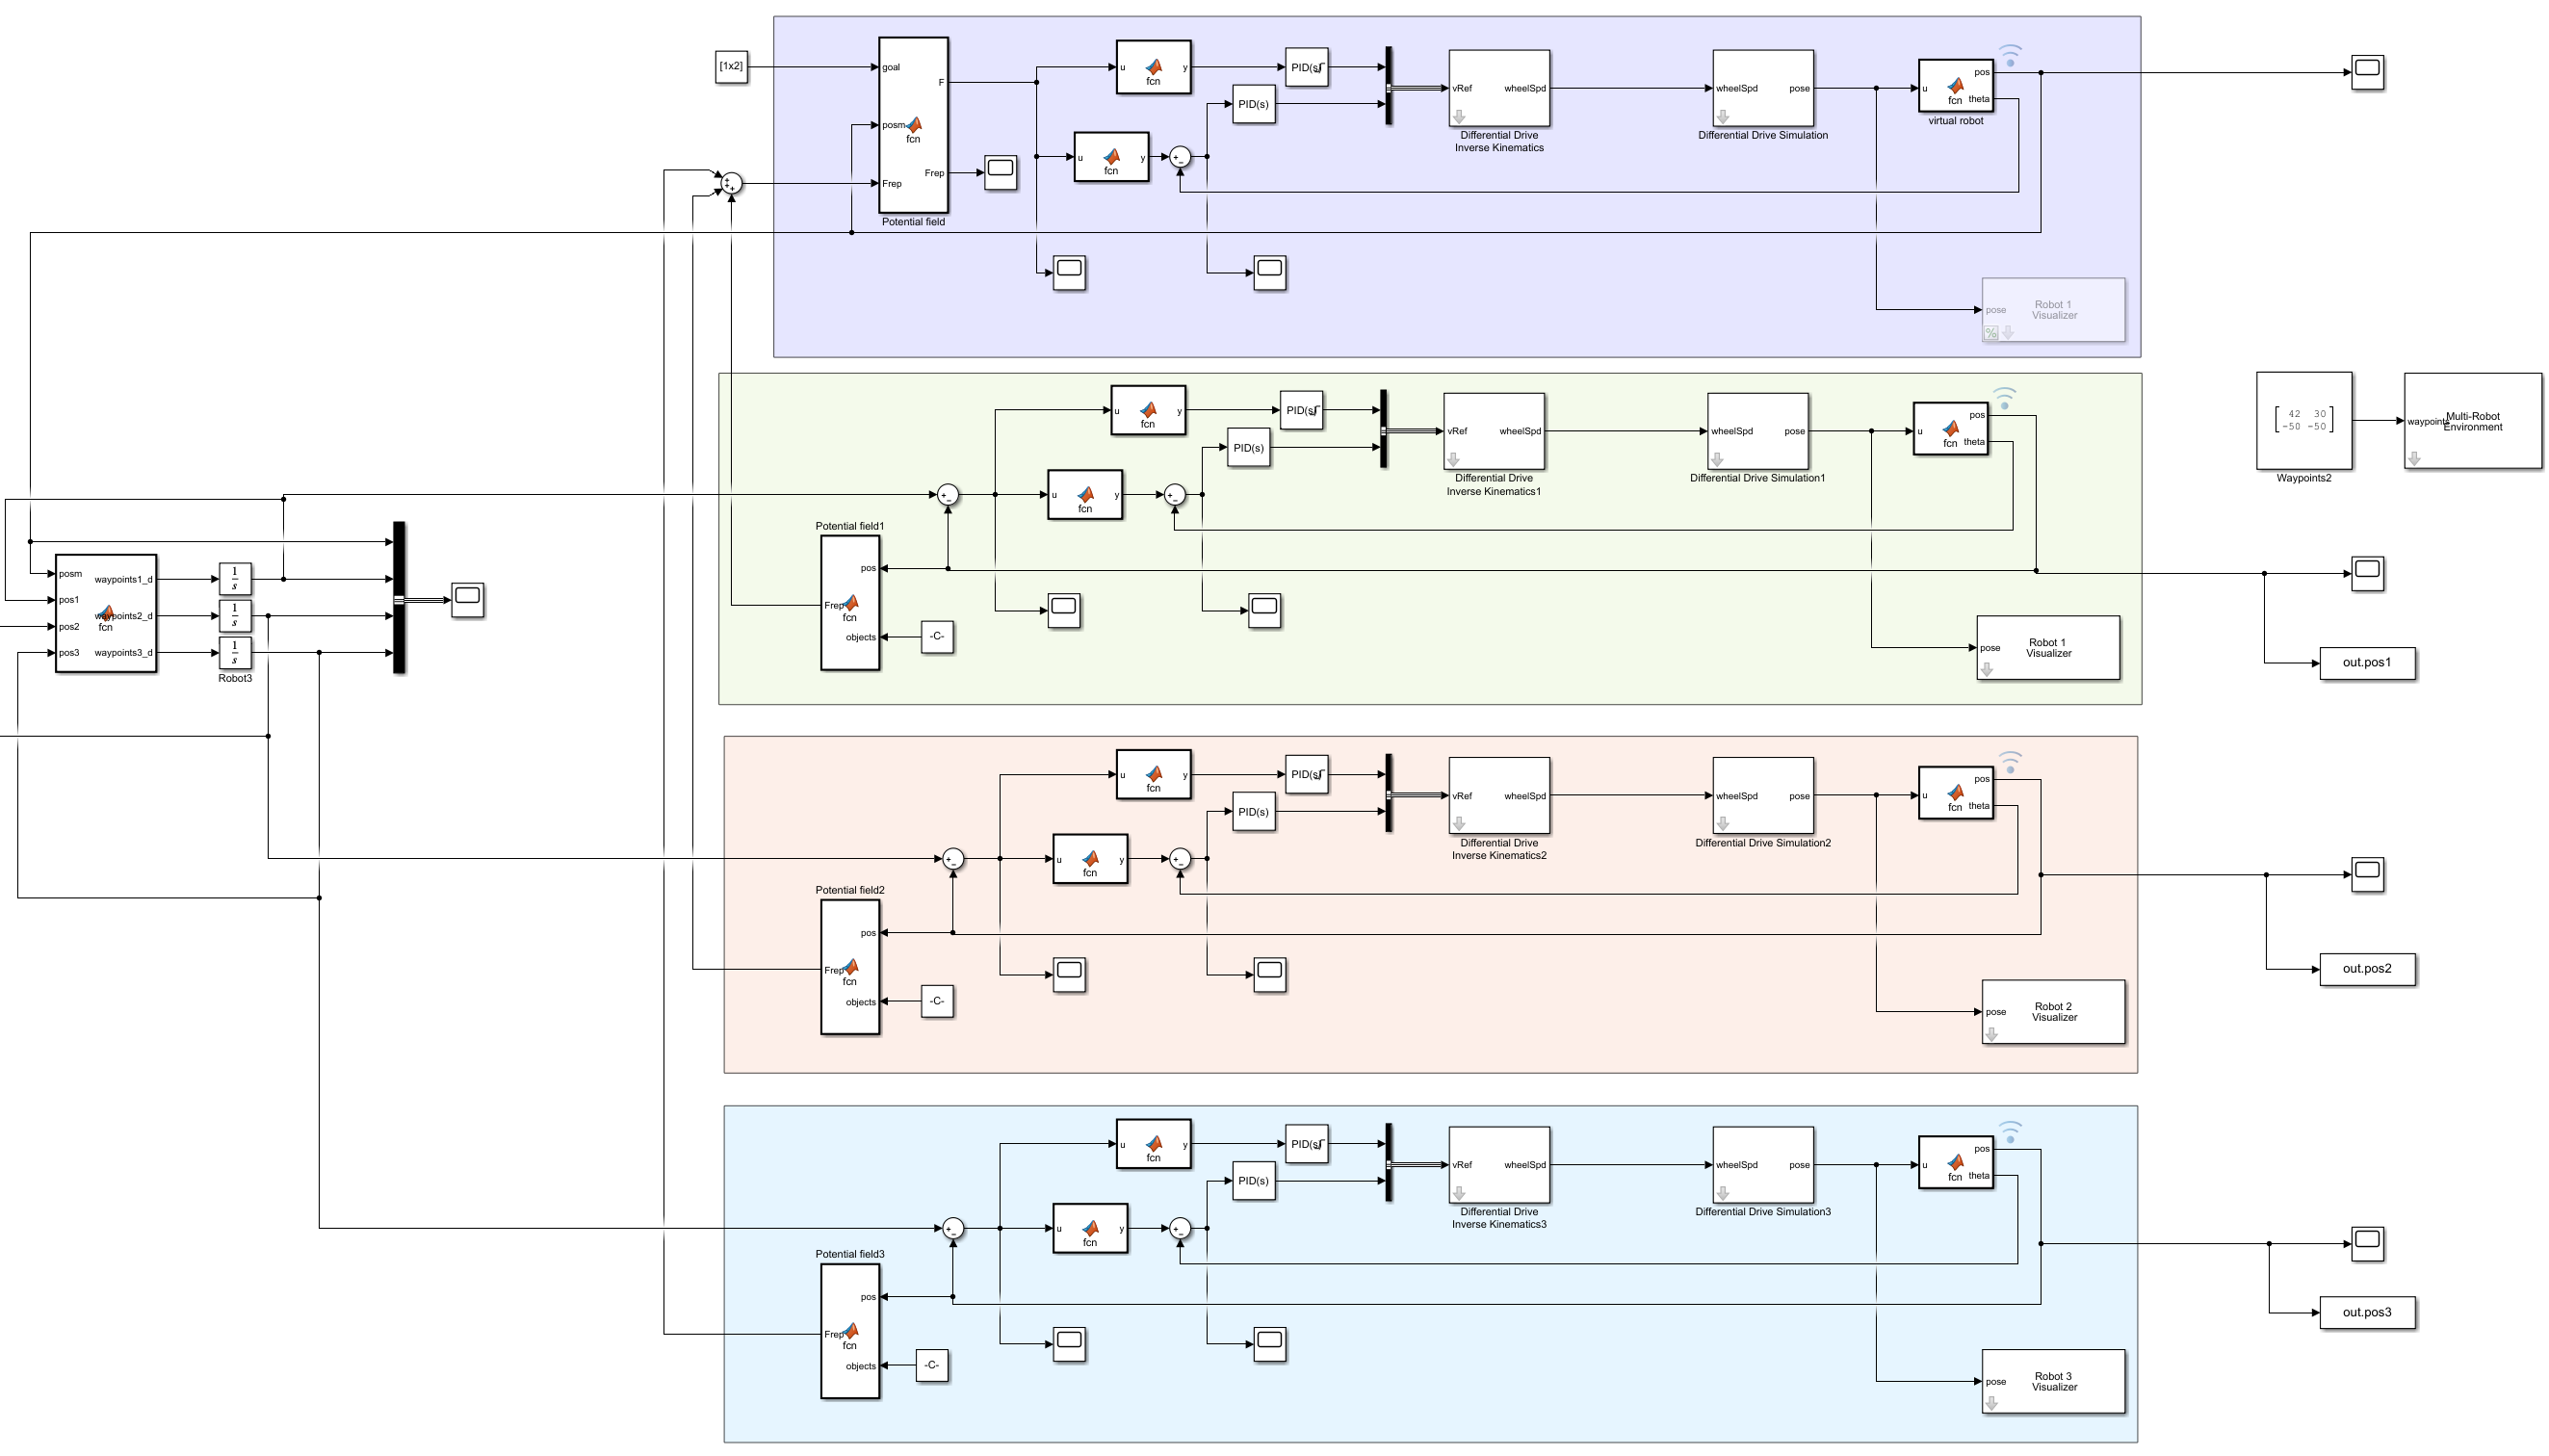
\includegraphics[scale=0.25]{Images/platoon-potential-field-distributed-simulink.png}
	\caption{بلوک‌های شبیه‌سازی در روش شکل‌گیری ثابت با محاسبات نامتمرکز}\label{Fig platoon-potential-field-distributed-simulink}
\end{figure}


مکان ربات‌ها برای روش نامتمرکز در شکل \ref{Fig platoon-potential-field-distributed-pos} به نمایش در آمده است.
\begin{figure}[!h]
	\centering
	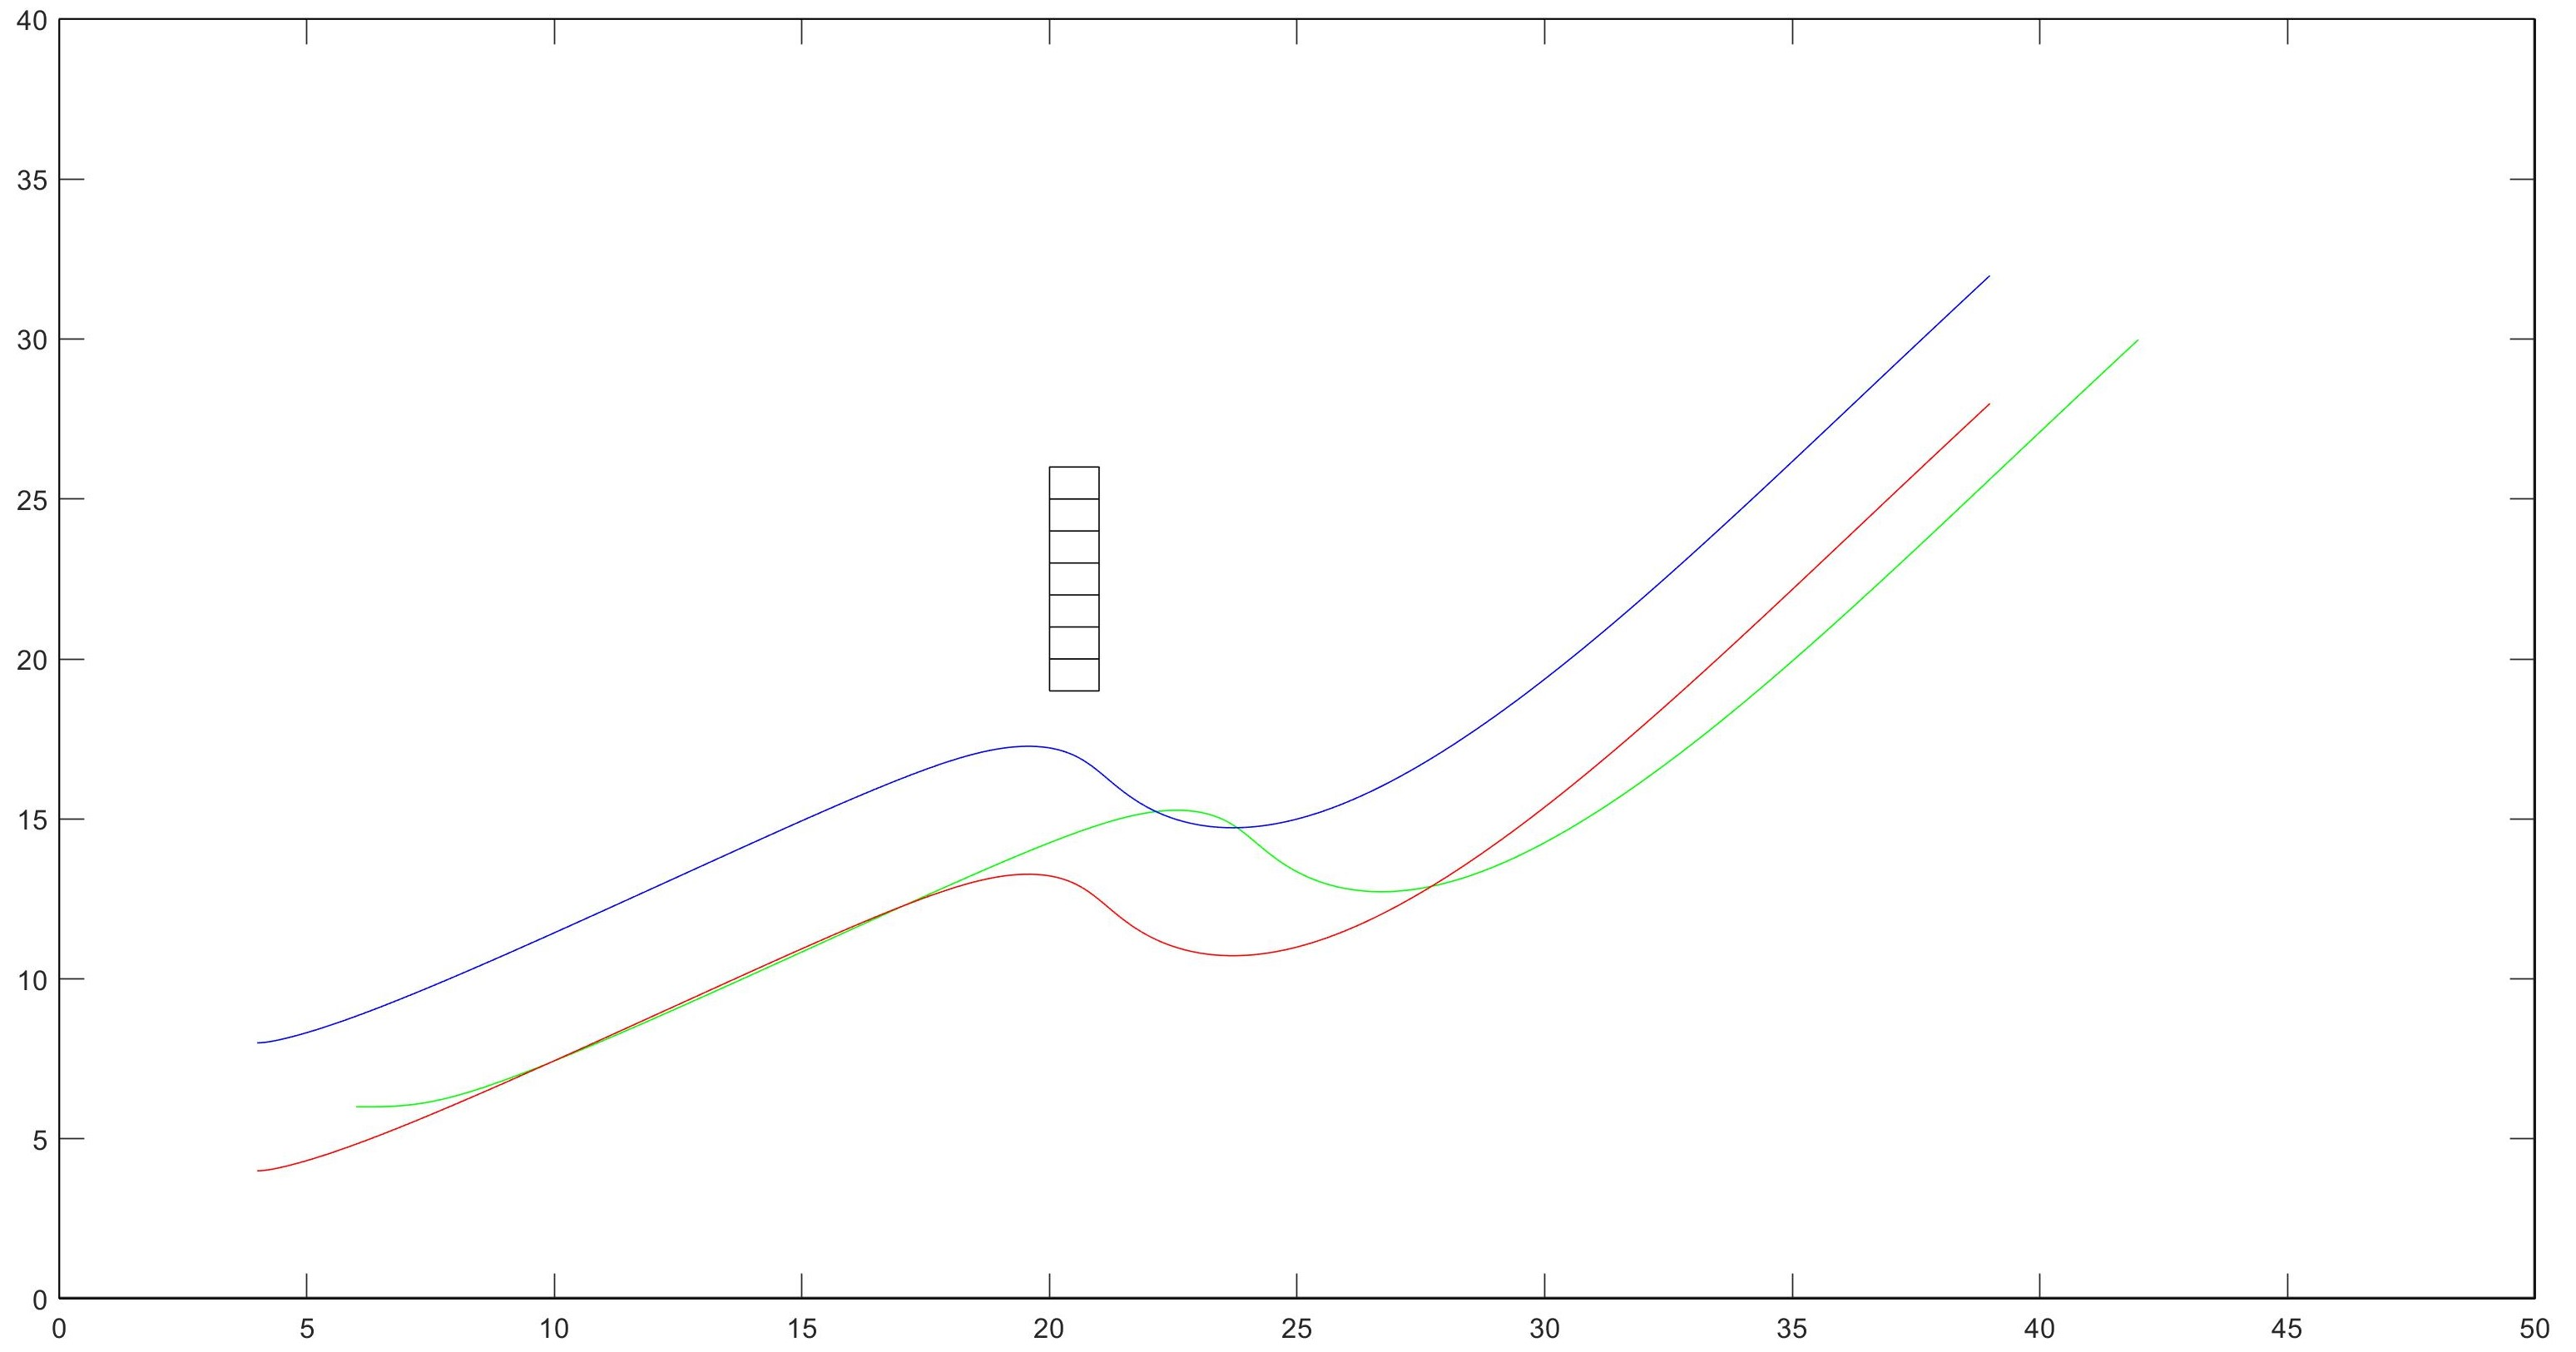
\includegraphics[scale=0.2]{Images/platoon-potential-field-distributed-pos.jpg}
	\caption{مکان ربات‌ها در روش شکل‌گیری ثابت با محاسبات نامتمرکز}\label{Fig platoon-potential-field-distributed-pos}
\end{figure}


مشکل اصلی این روش این است که امکان دارد هر ربات از جهت مختلفی به طور همزمان به مانع نزدیک شوند، مخصوصا در شرایطی که مانع متحرک باشد، لذا نیاز داریم هر ربات به تنهایی میدان پتانسیل مخصوص به خود را داشته باشد. که در قسمت بعد این ایده پیاده‌سازی گشته است.

\subsection{جلوگیری از برخورد با موانع با شکل‌گیری شکننده}\label{sec potential-field for every robot}
در این روش هر ربات با میدان پتانسیل مخصوص به خود مسیریابی را انجام می‌دهد و نقطه‌ای که در هر لحظه باید در اجماع قرار گیرد به عنوان نقطه هدف در نظر گرفته می‌شود. بلوک‌های شبیه‌سازی در شکل \ref{Fig platoon-potential-field-independent-simulink} و نتیجه حرکت ربات‌ها در شکل \ref{Fig platoon-potential-field-independent-pos} به نمایش در آمده است.
\begin{figure}[!h]
	\centering
	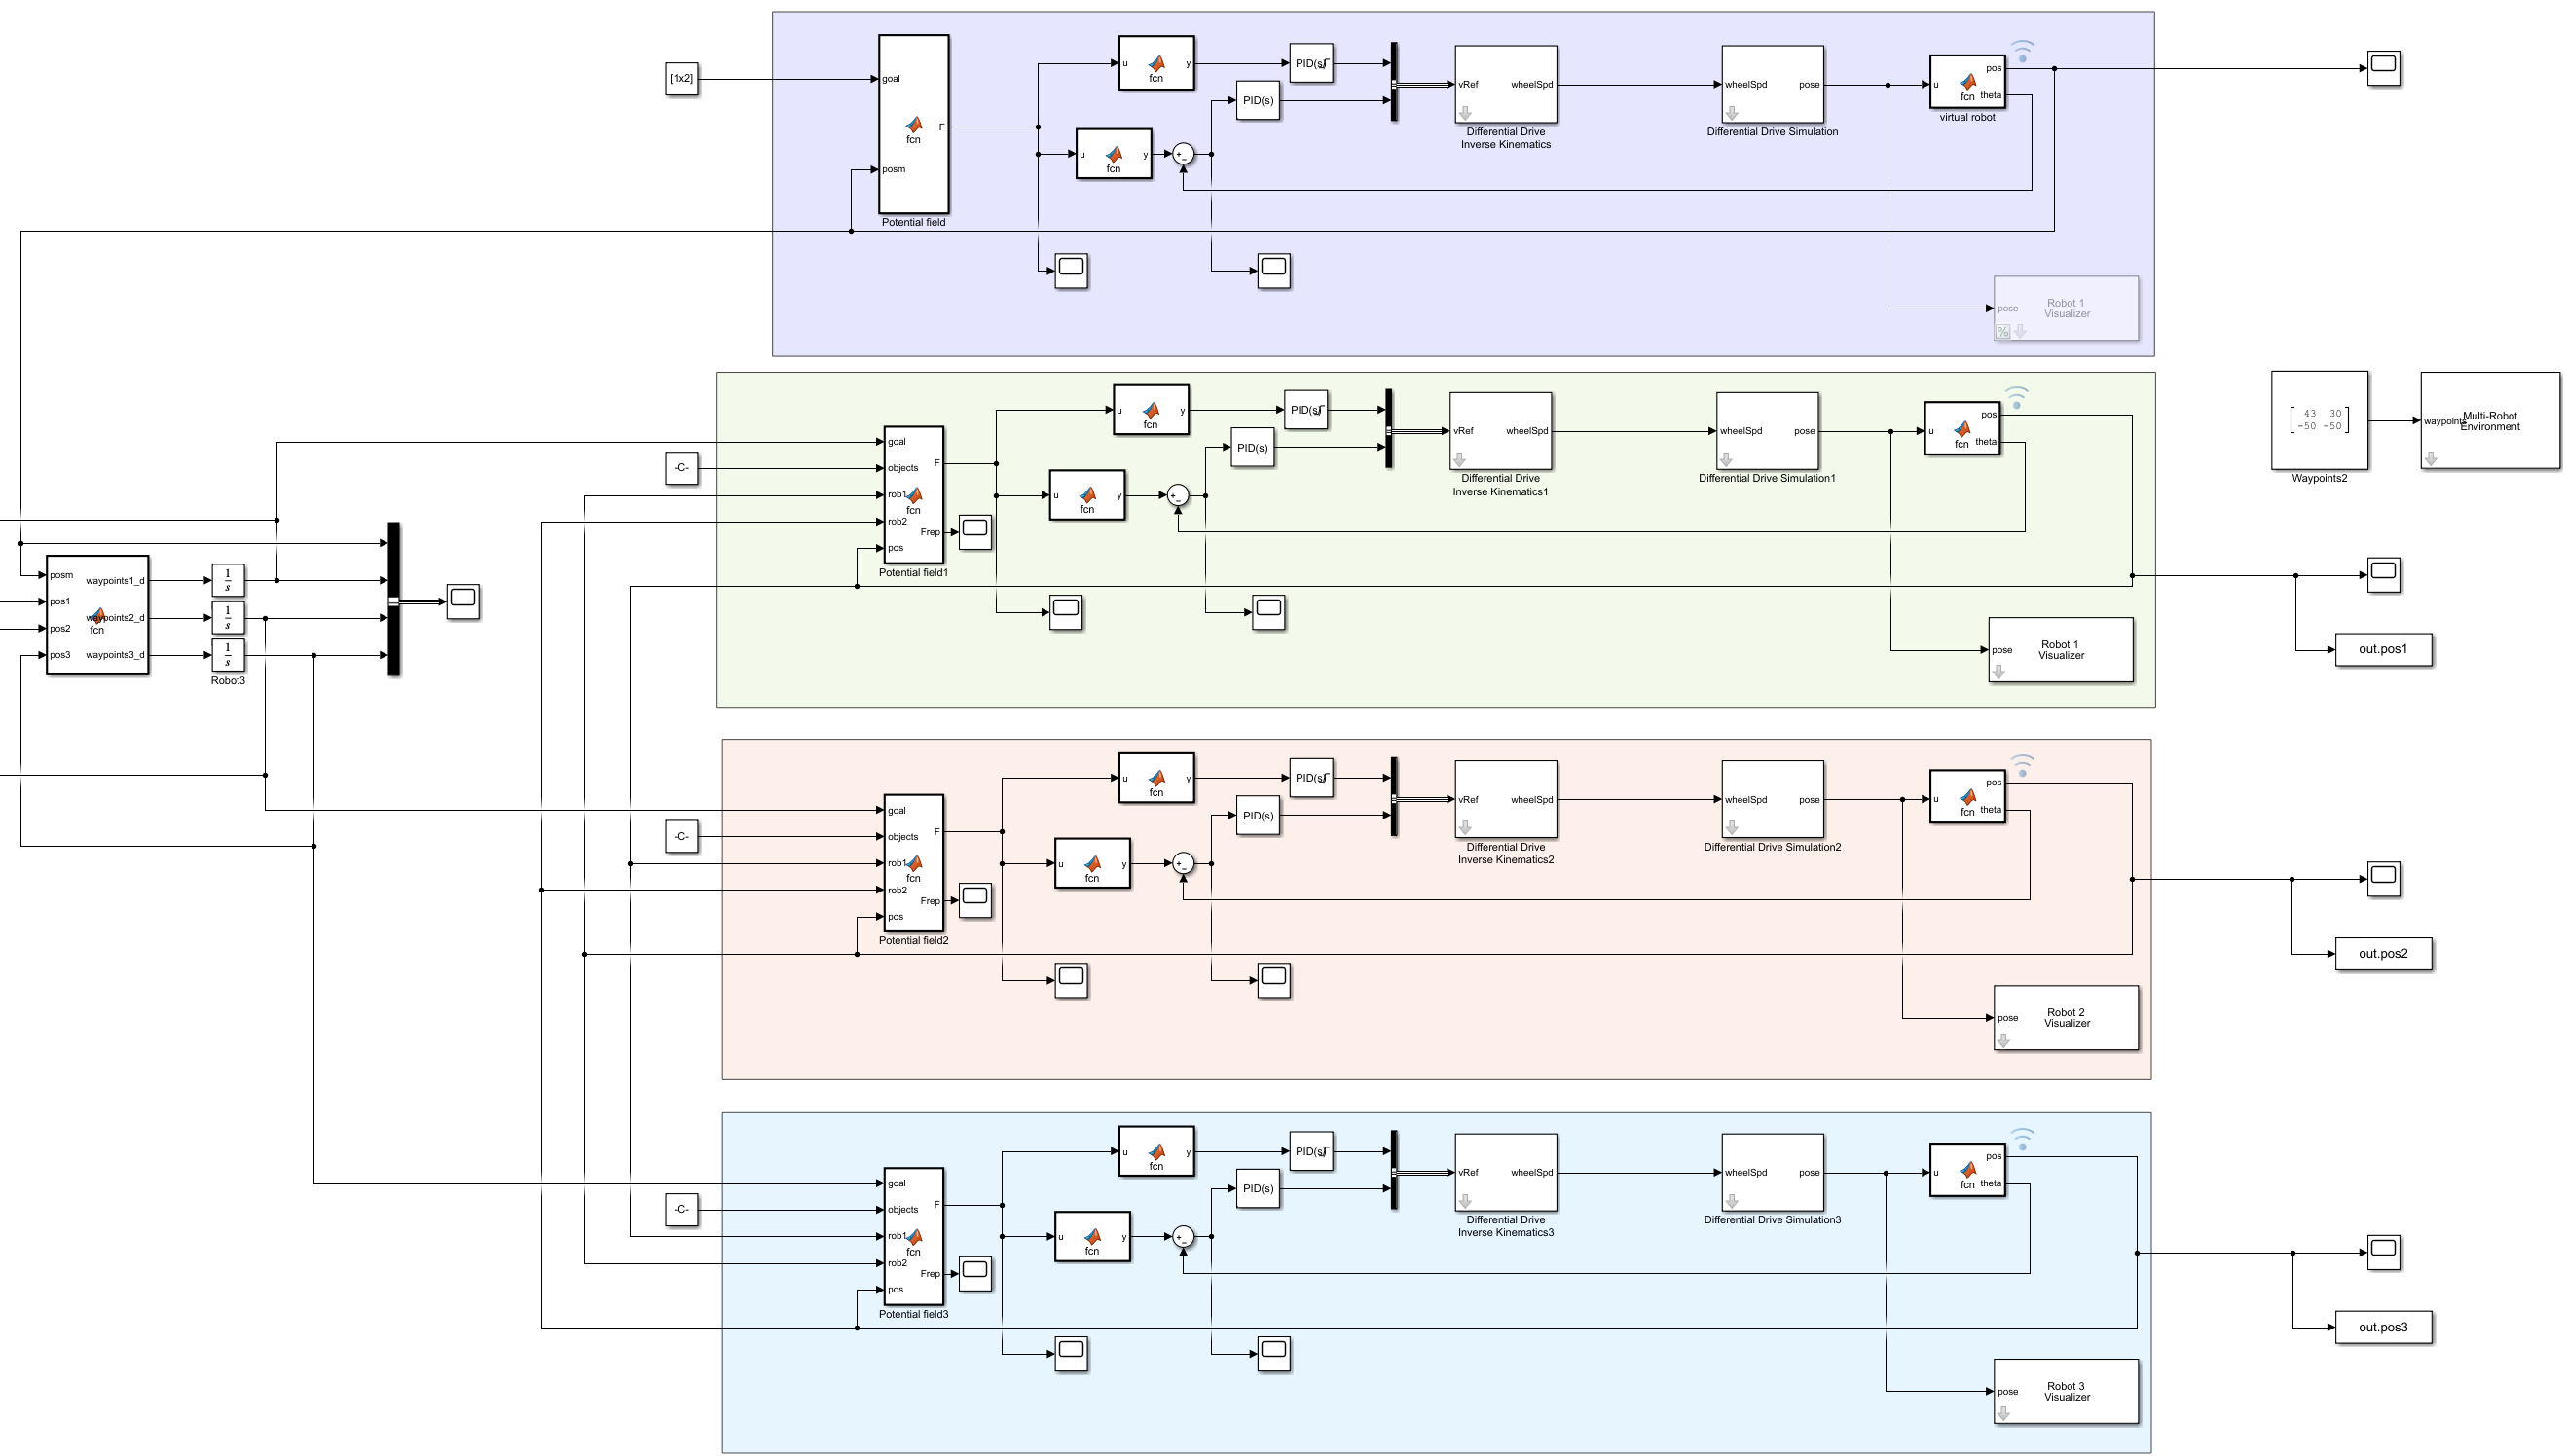
\includegraphics[scale=0.2]{Images/platoon-potential-field-independent-simulink.png}
	\caption{بلوک‌های شبیه‌سازی در روش شکل‌گیری شکننده}\label{Fig platoon-potential-field-independent-simulink}
\end{figure}

\begin{figure}[!h]
	\centering
	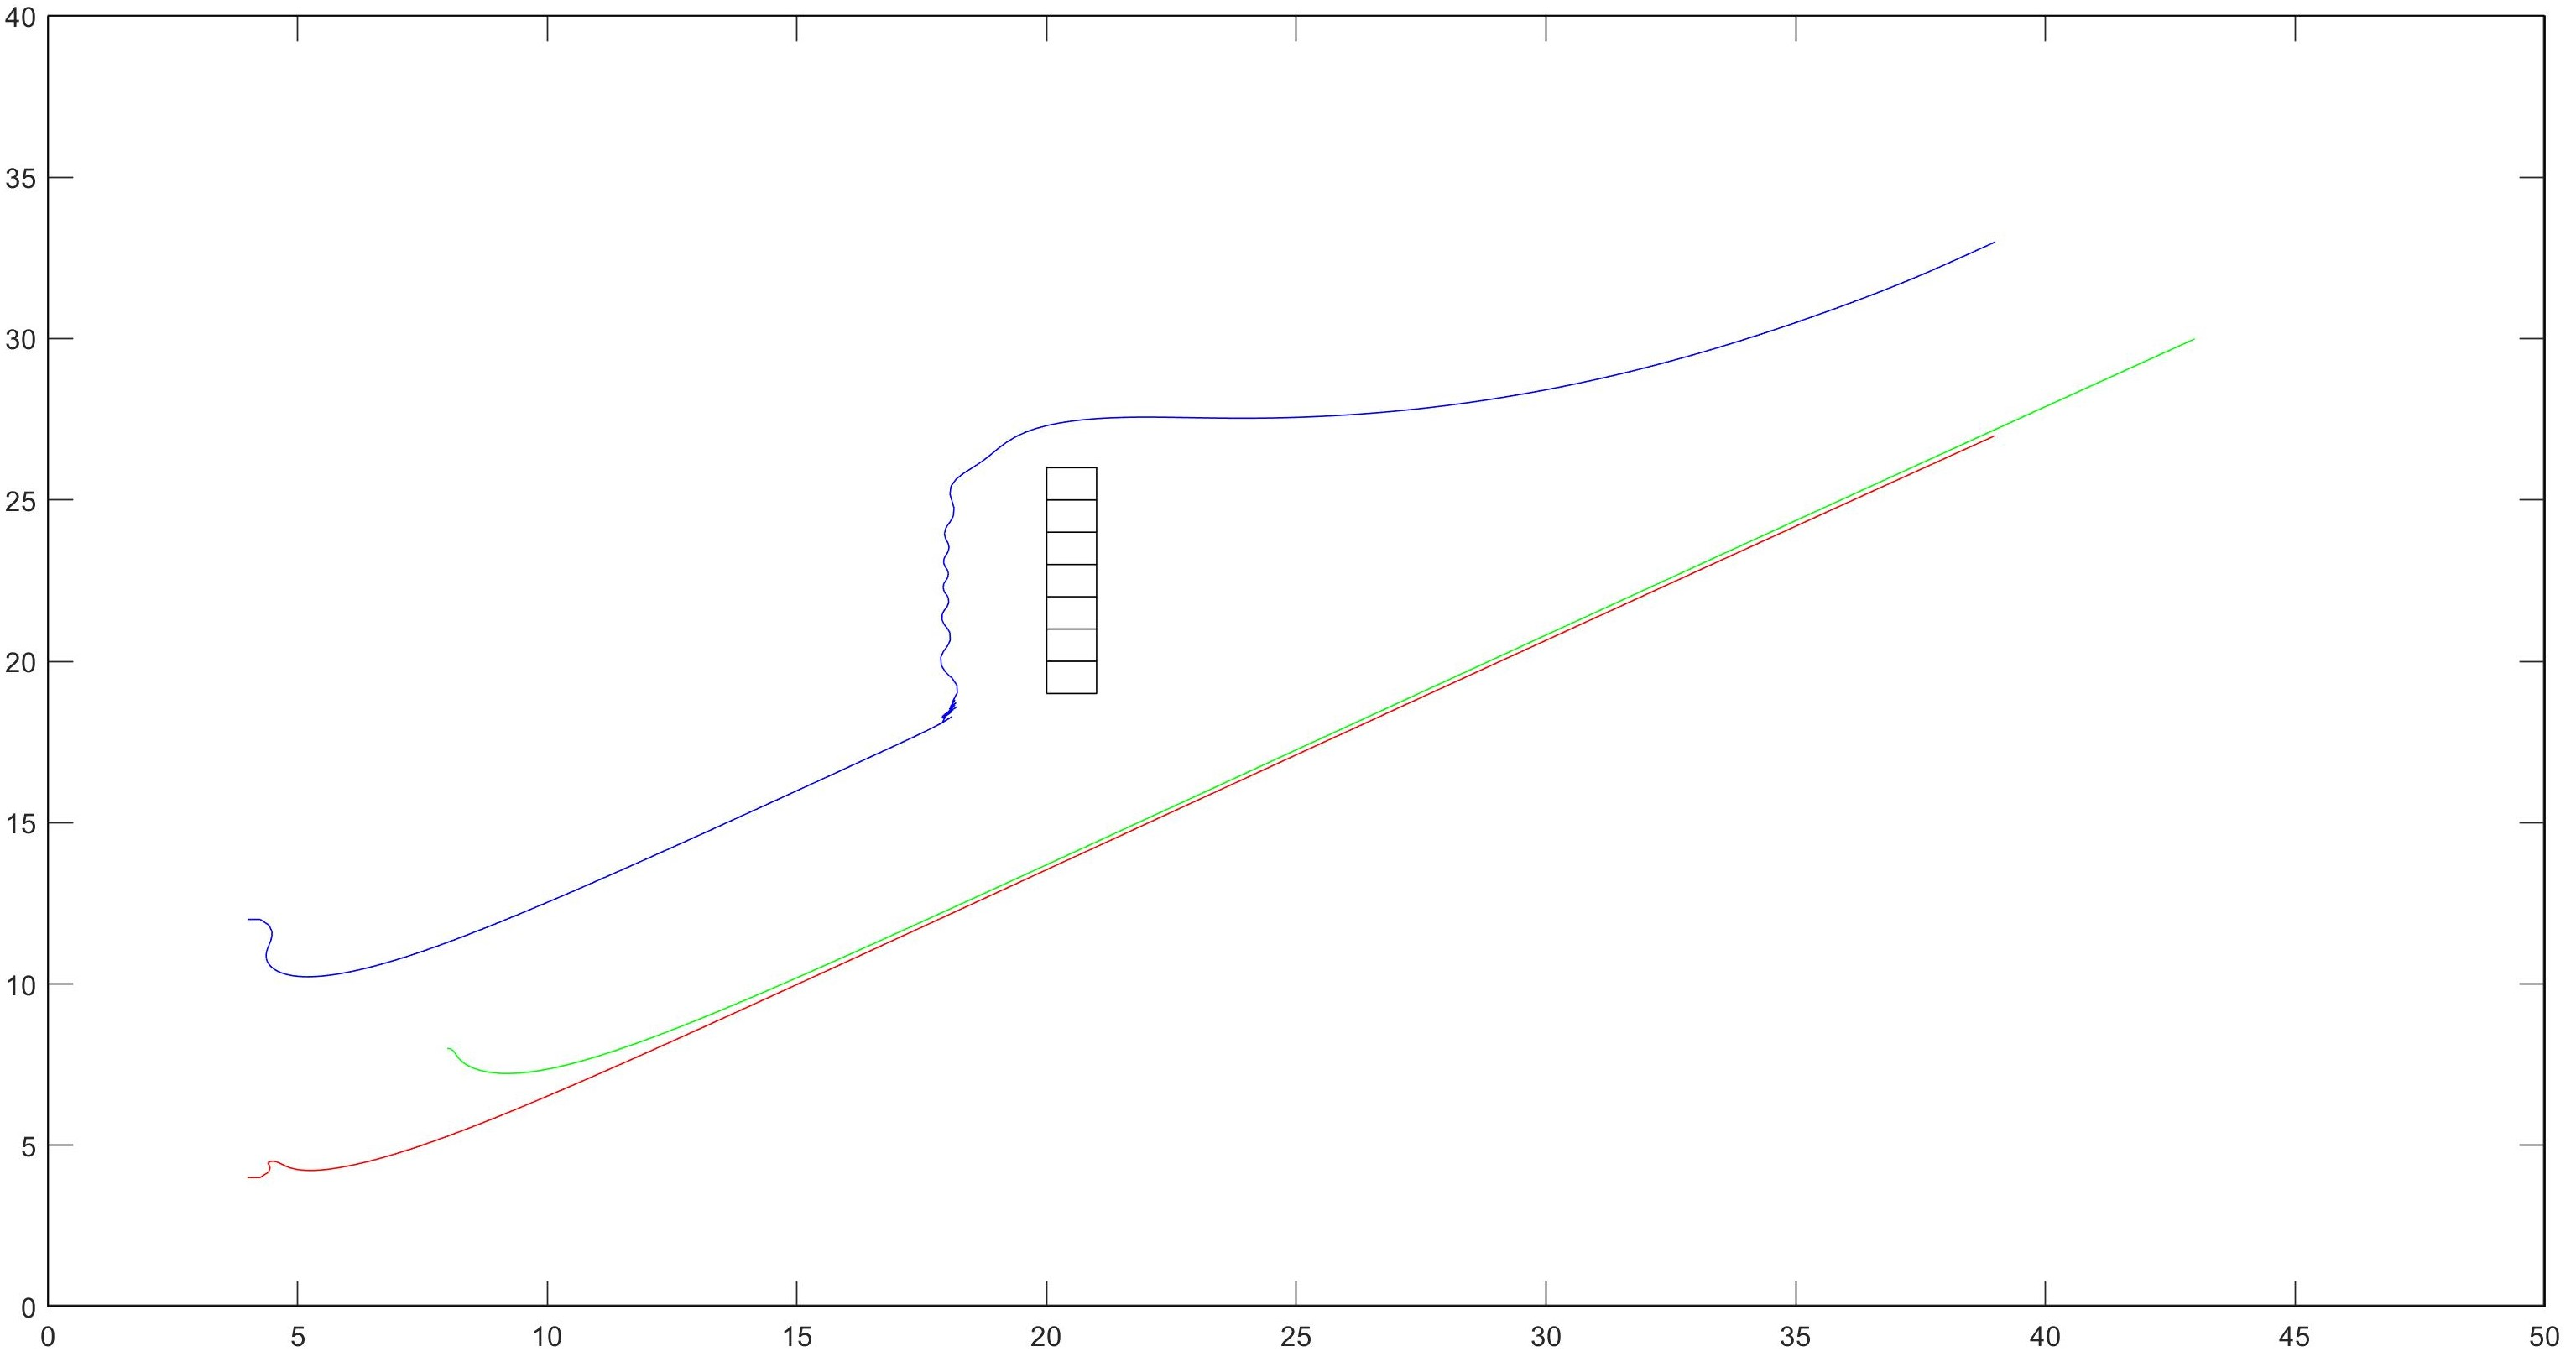
\includegraphics[scale=0.2]{Images/platoon-potential-field-independent-pos.jpg}
	\caption{مکان ربات‌ها در روش شکل‌گیری شکننده}\label{Fig platoon-potential-field-independent-pos}
\end{figure}



\section{روش‌های ابتکاری}
در این قسمت روش‌های ابتکاری فصل \ref{ch path planning} پیاده‌سازی شده‌اند. این مسیریابی‌ها به صورت آنلاین انجام شده است تا از برخورد با موانع متحرک نیز بتوان اجتناب کرد. روش پیاده‌سازی به این صورت است که در عامل رهبر، این مسیریابی انجام و ربات طبق آن حرکت می‌نماید. سایر ربات‌ها همانند بخش \ref{sec potential-field for every robot} از میدان پتانسیل برای رسیدن به مکان مطلوب تعیین شده از طرف کنترل‌کننده پلتون و دوری از موانع به صورت انفرادی، استفاده می‌کنند.

\subsection{$BFS$}
نحوه پیاده‌سازی مسیریابی $BFS$ توسط اجماع ربات‌ها در شکل \ref{Fig platoon-BSF-simulink} و مسیر پیموده شده در شکل \ref{Fig platoon-BSF-pos} قابل مشاهده است.
\begin{figure}[!h]
	\centering
	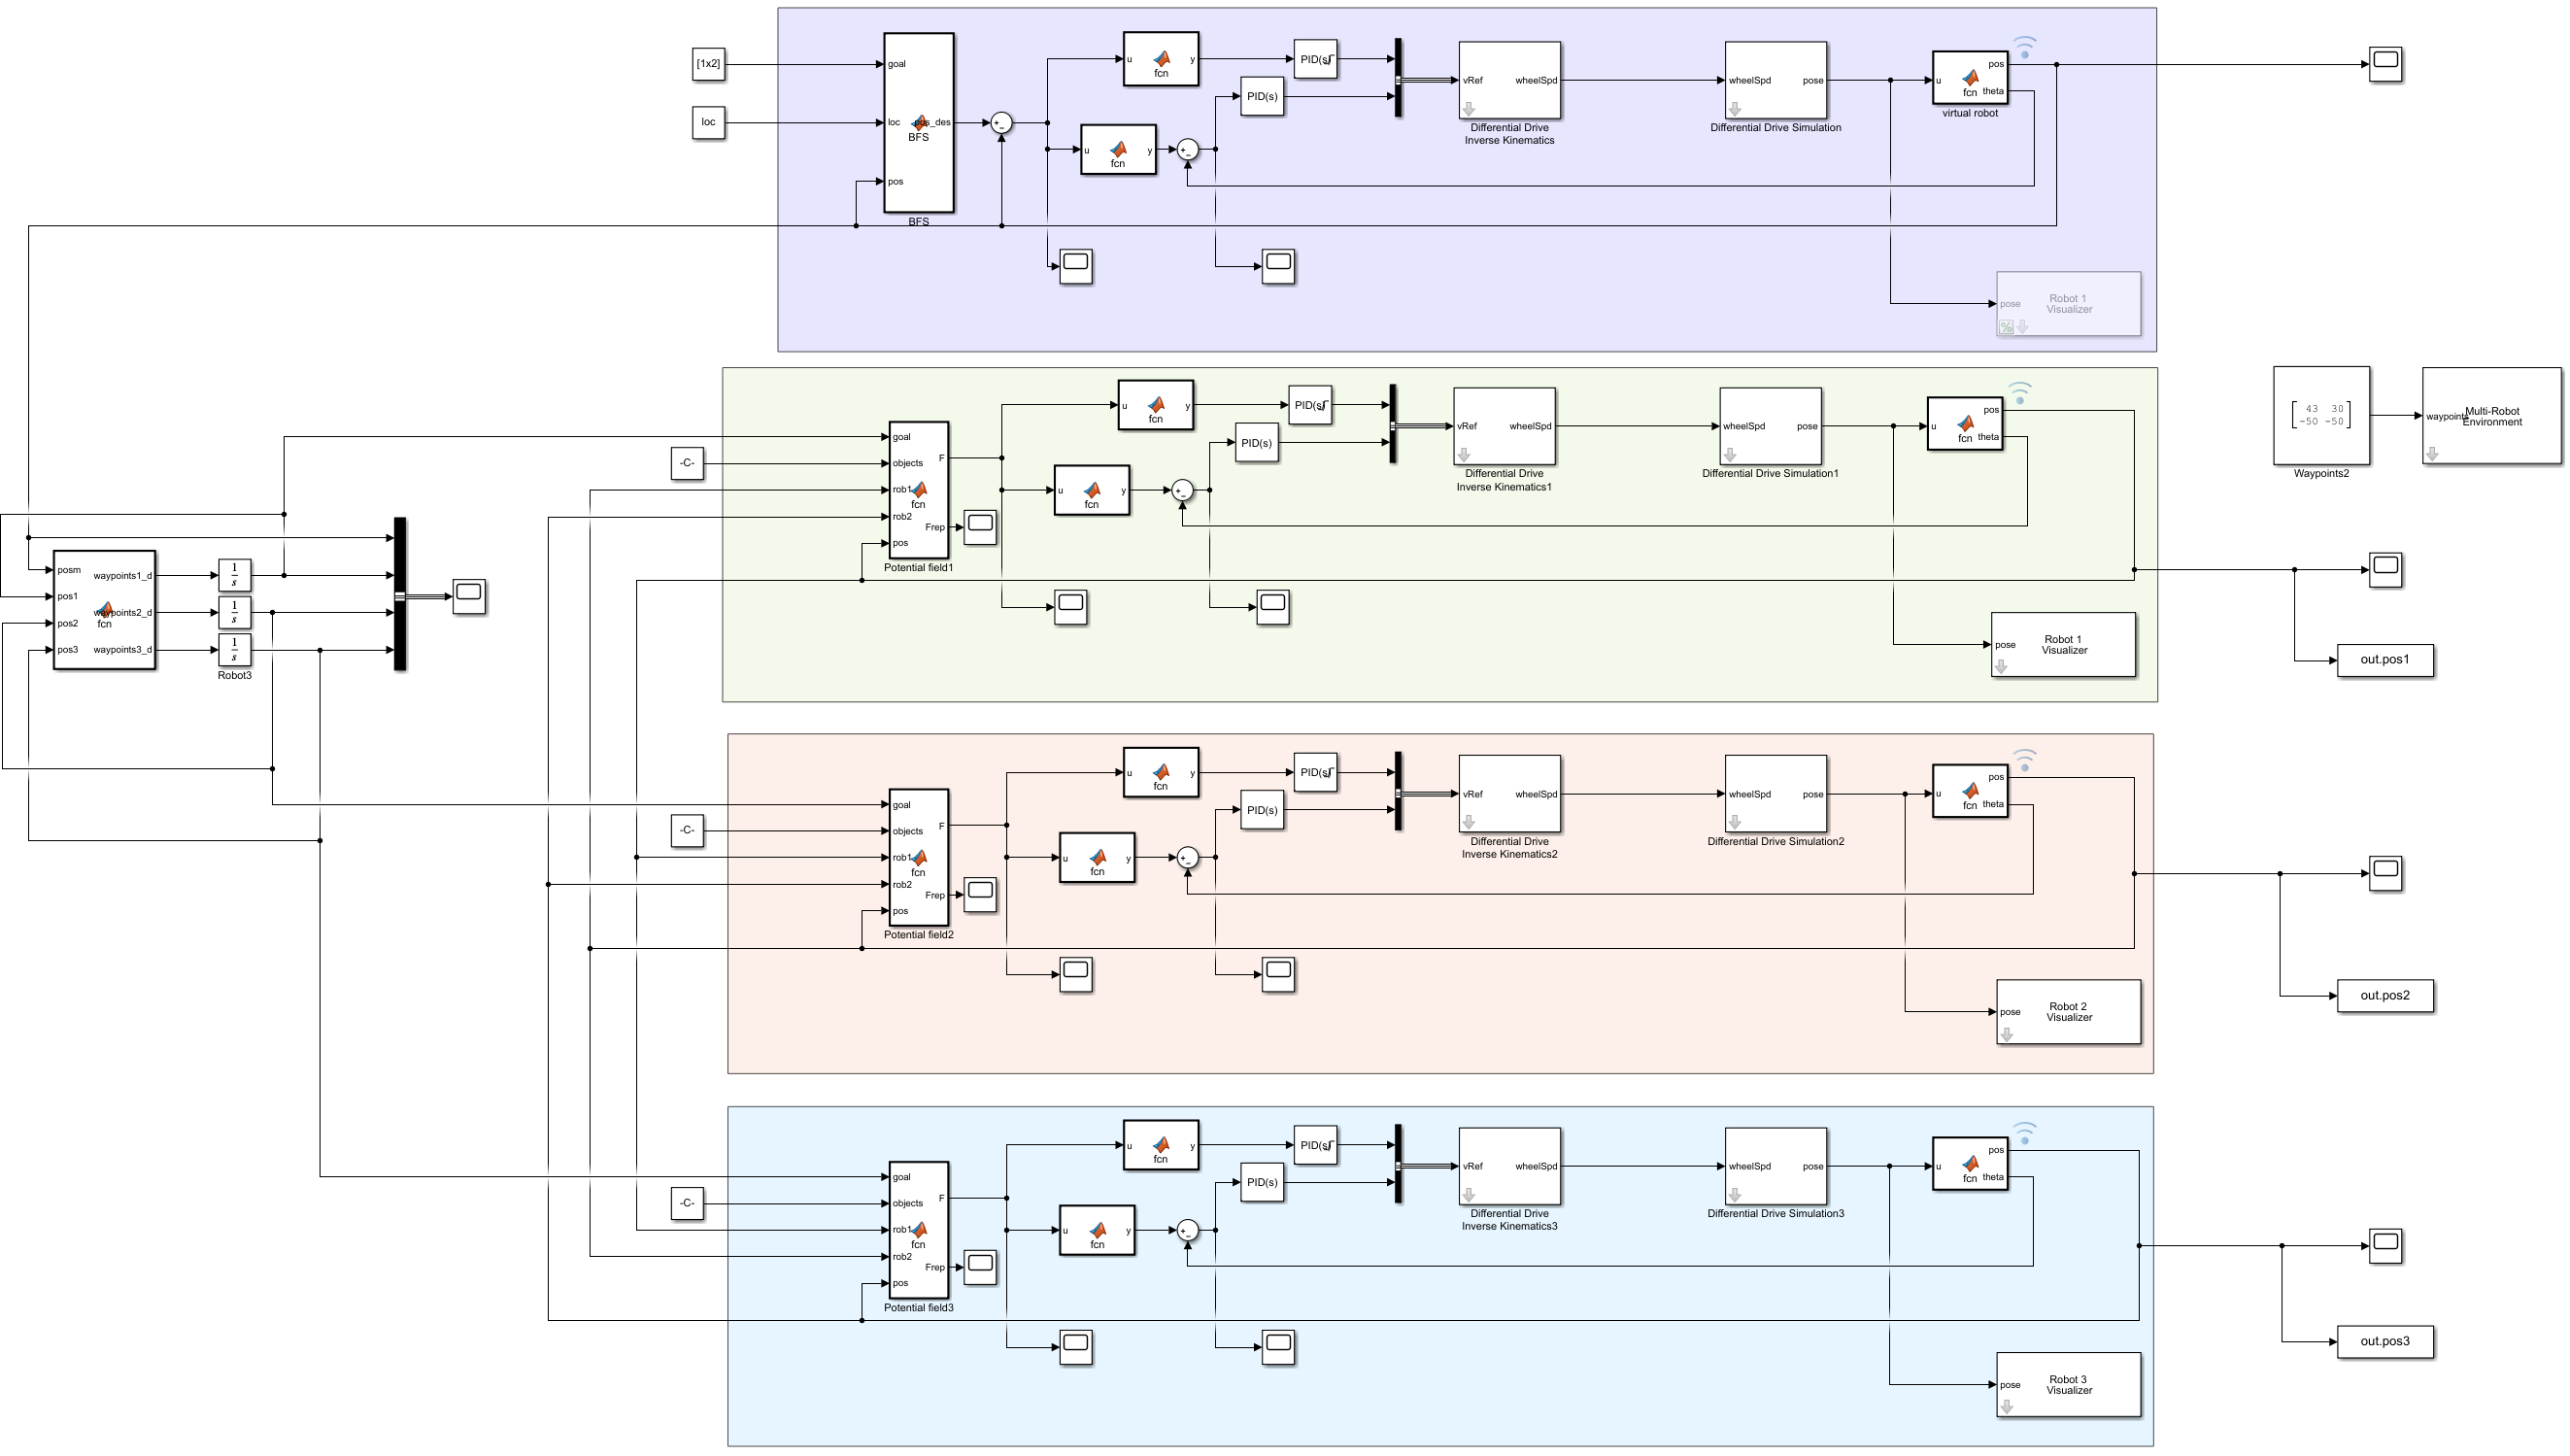
\includegraphics[scale=0.22]{Images/platoon-BFS-simulink.png}
	\caption{بلوک‌های شبیه‌سازی در روش $BFS$}\label{Fig platoon-BSF-simulink}
\end{figure}

\begin{figure}[!h]
	\centering
	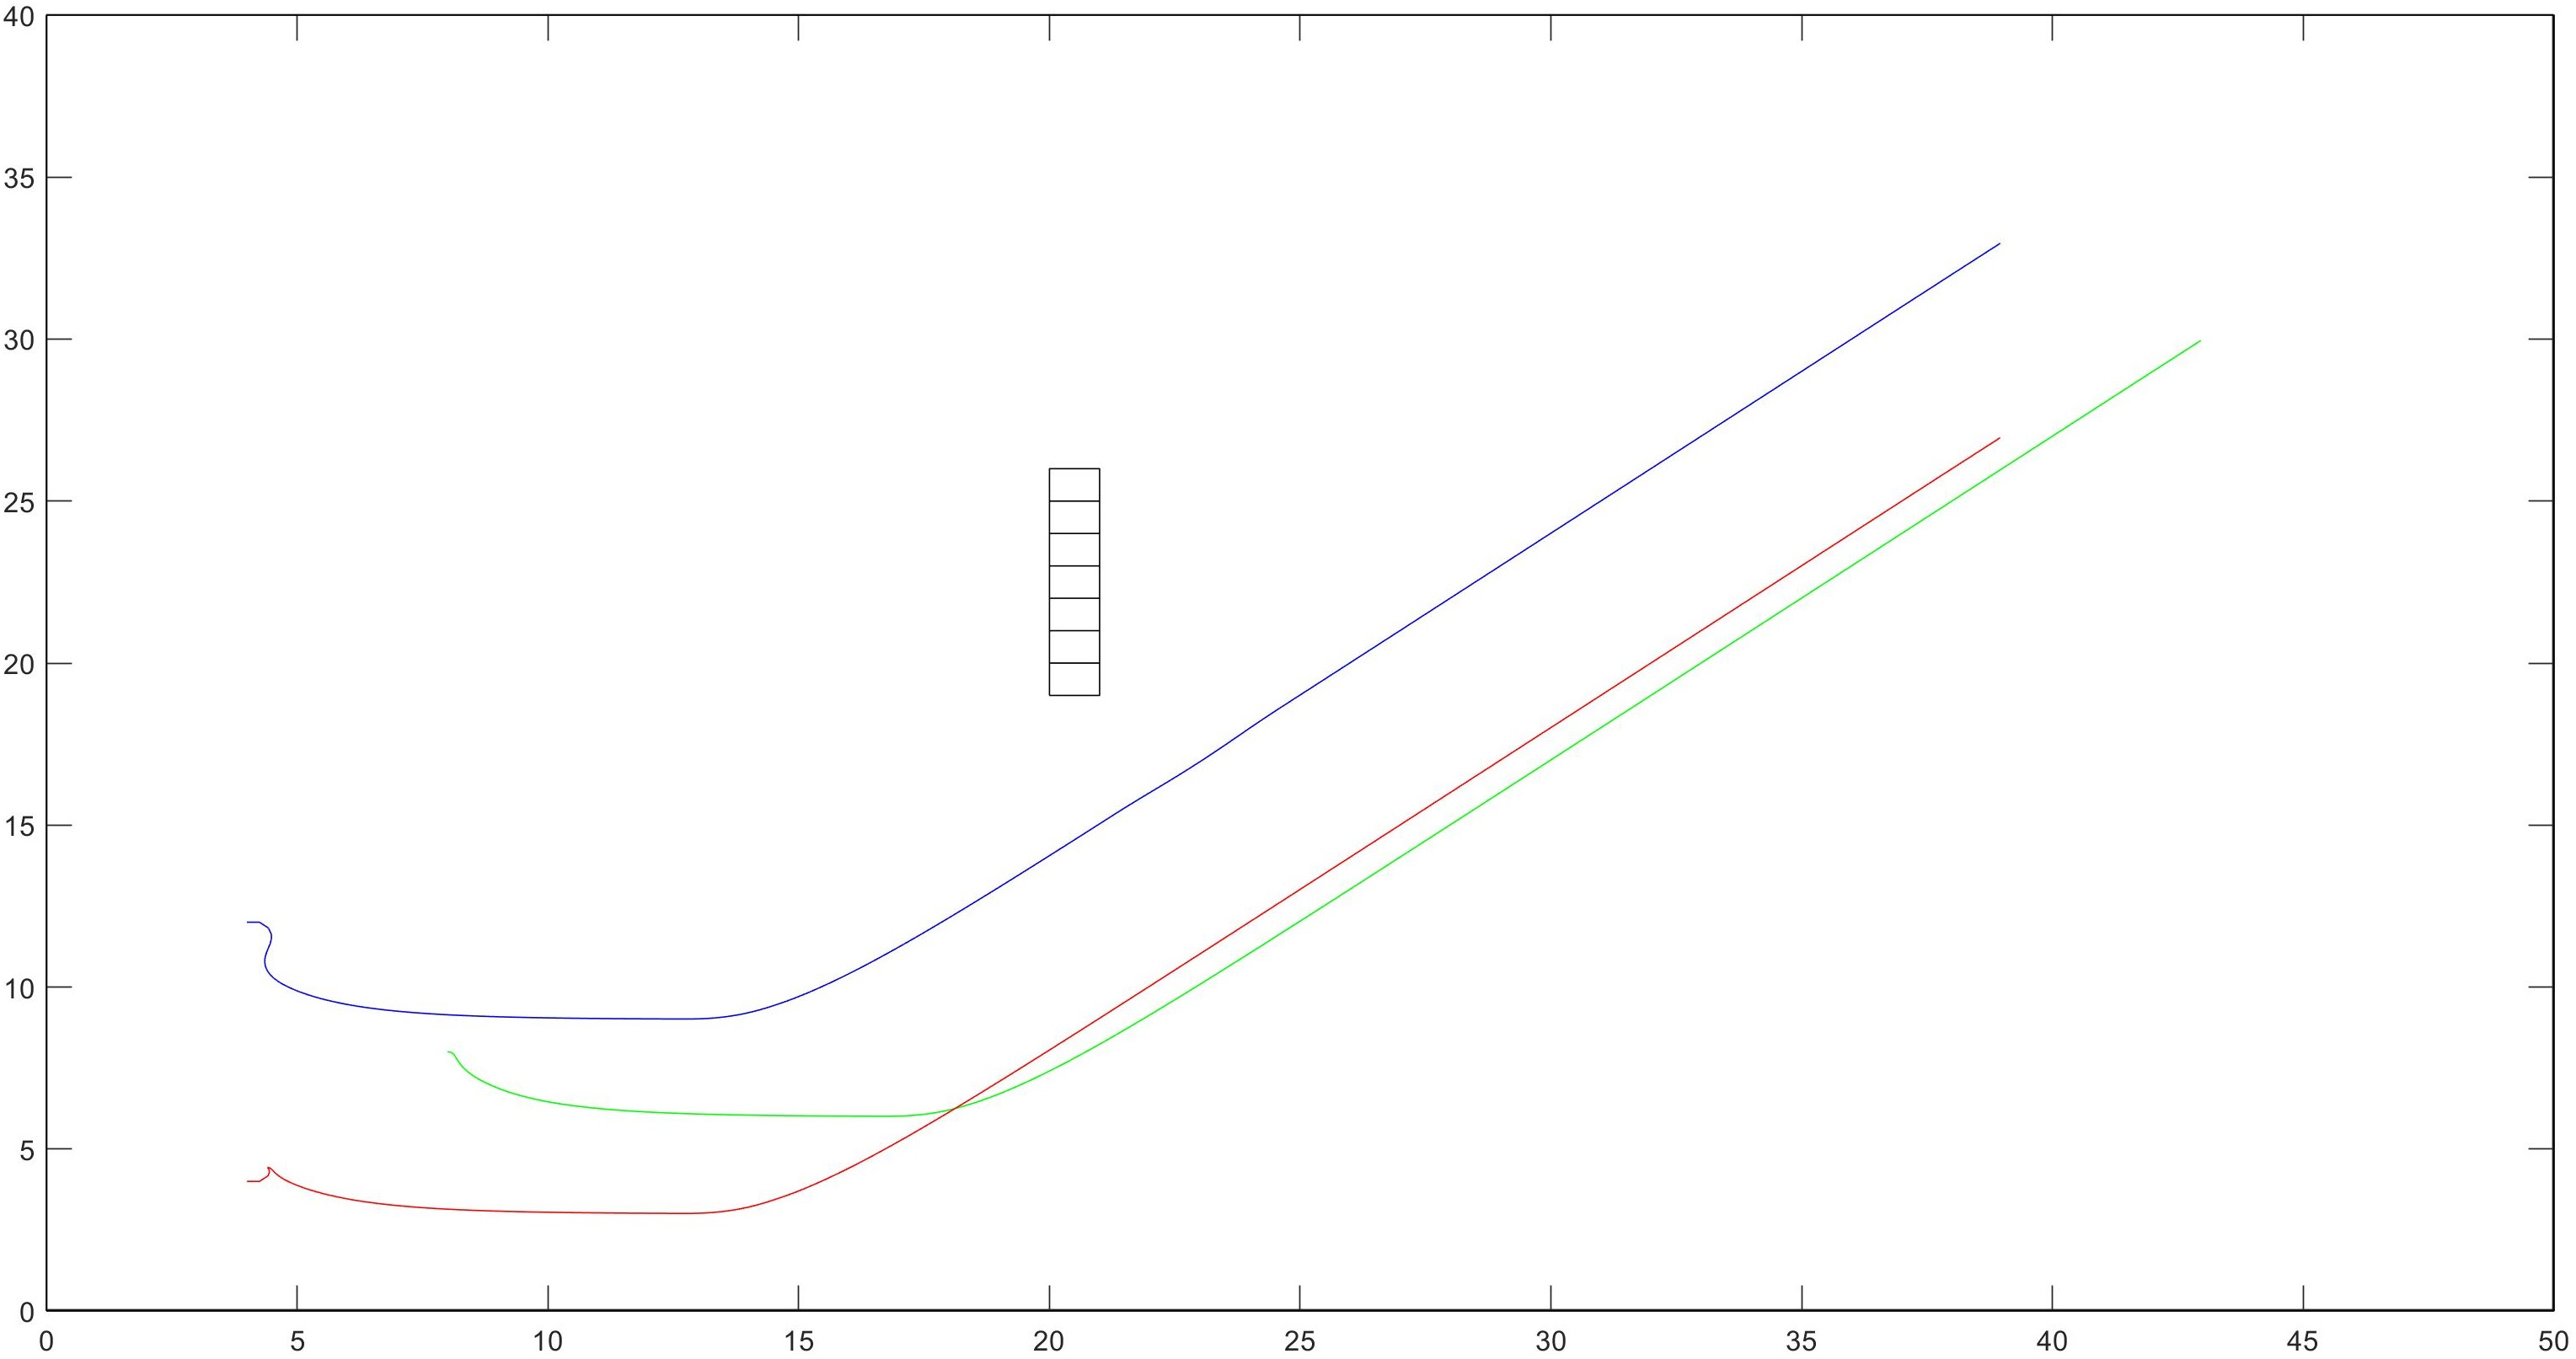
\includegraphics[scale=0.2]{Images/platoon-BFS-pos.jpg}
	\caption{مکان ربات‌ها در روش $BFS$}\label{Fig platoon-BSF-pos}
\end{figure}

\newpage
\subsection{$Greedy~best-first~search$}
پیاده‌سازی روش $Greedy~best-first~search$ برای مسیریابی اجماع ربات‌ها همراه با نتیجه‌ آن، به ترتیب در شکل‌های \ref{Fig platoon-Greedy-simulink} و \ref{Fig platoon-Greedy-pos} آمده است.
\begin{figure}[!h]
	\centering
	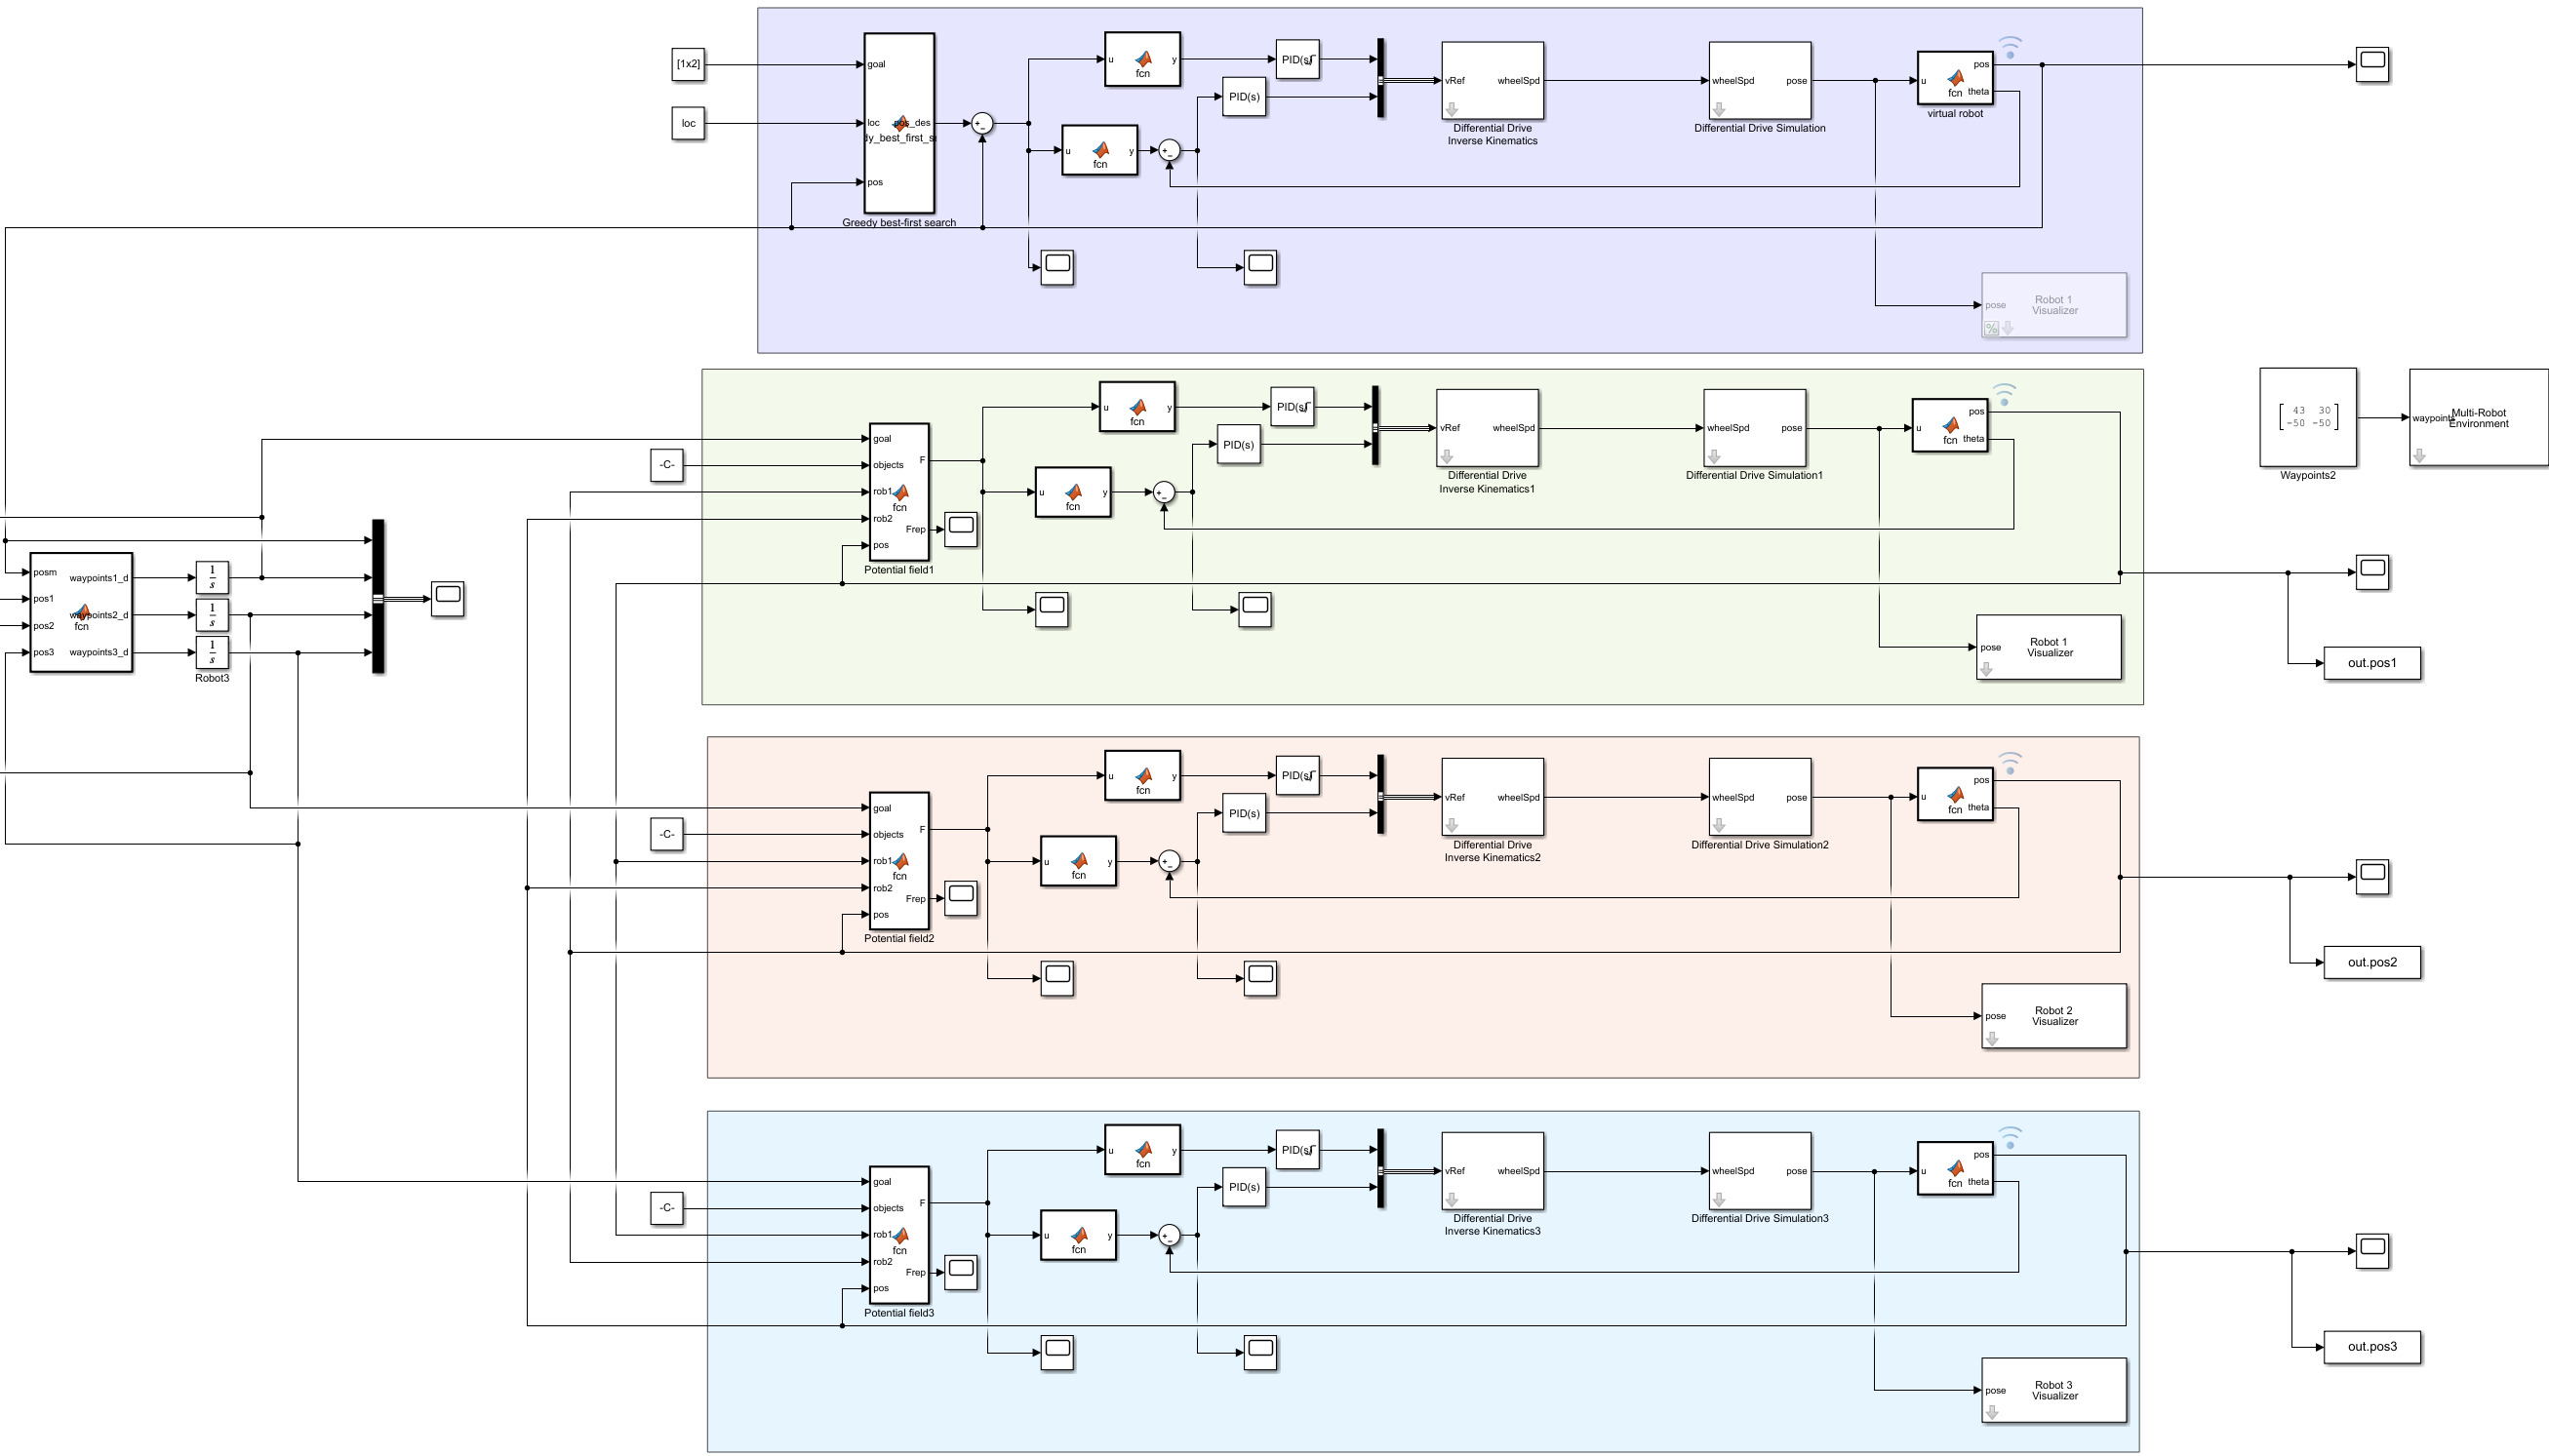
\includegraphics[scale=0.22]{Images/platoon-Greedy-simulink.png}
	\caption{بلوک‌های شبیه‌سازی در روش $Greedy~best-first~search$}\label{Fig platoon-Greedy-simulink}
\end{figure}

\begin{figure}[!h]
	\centering
	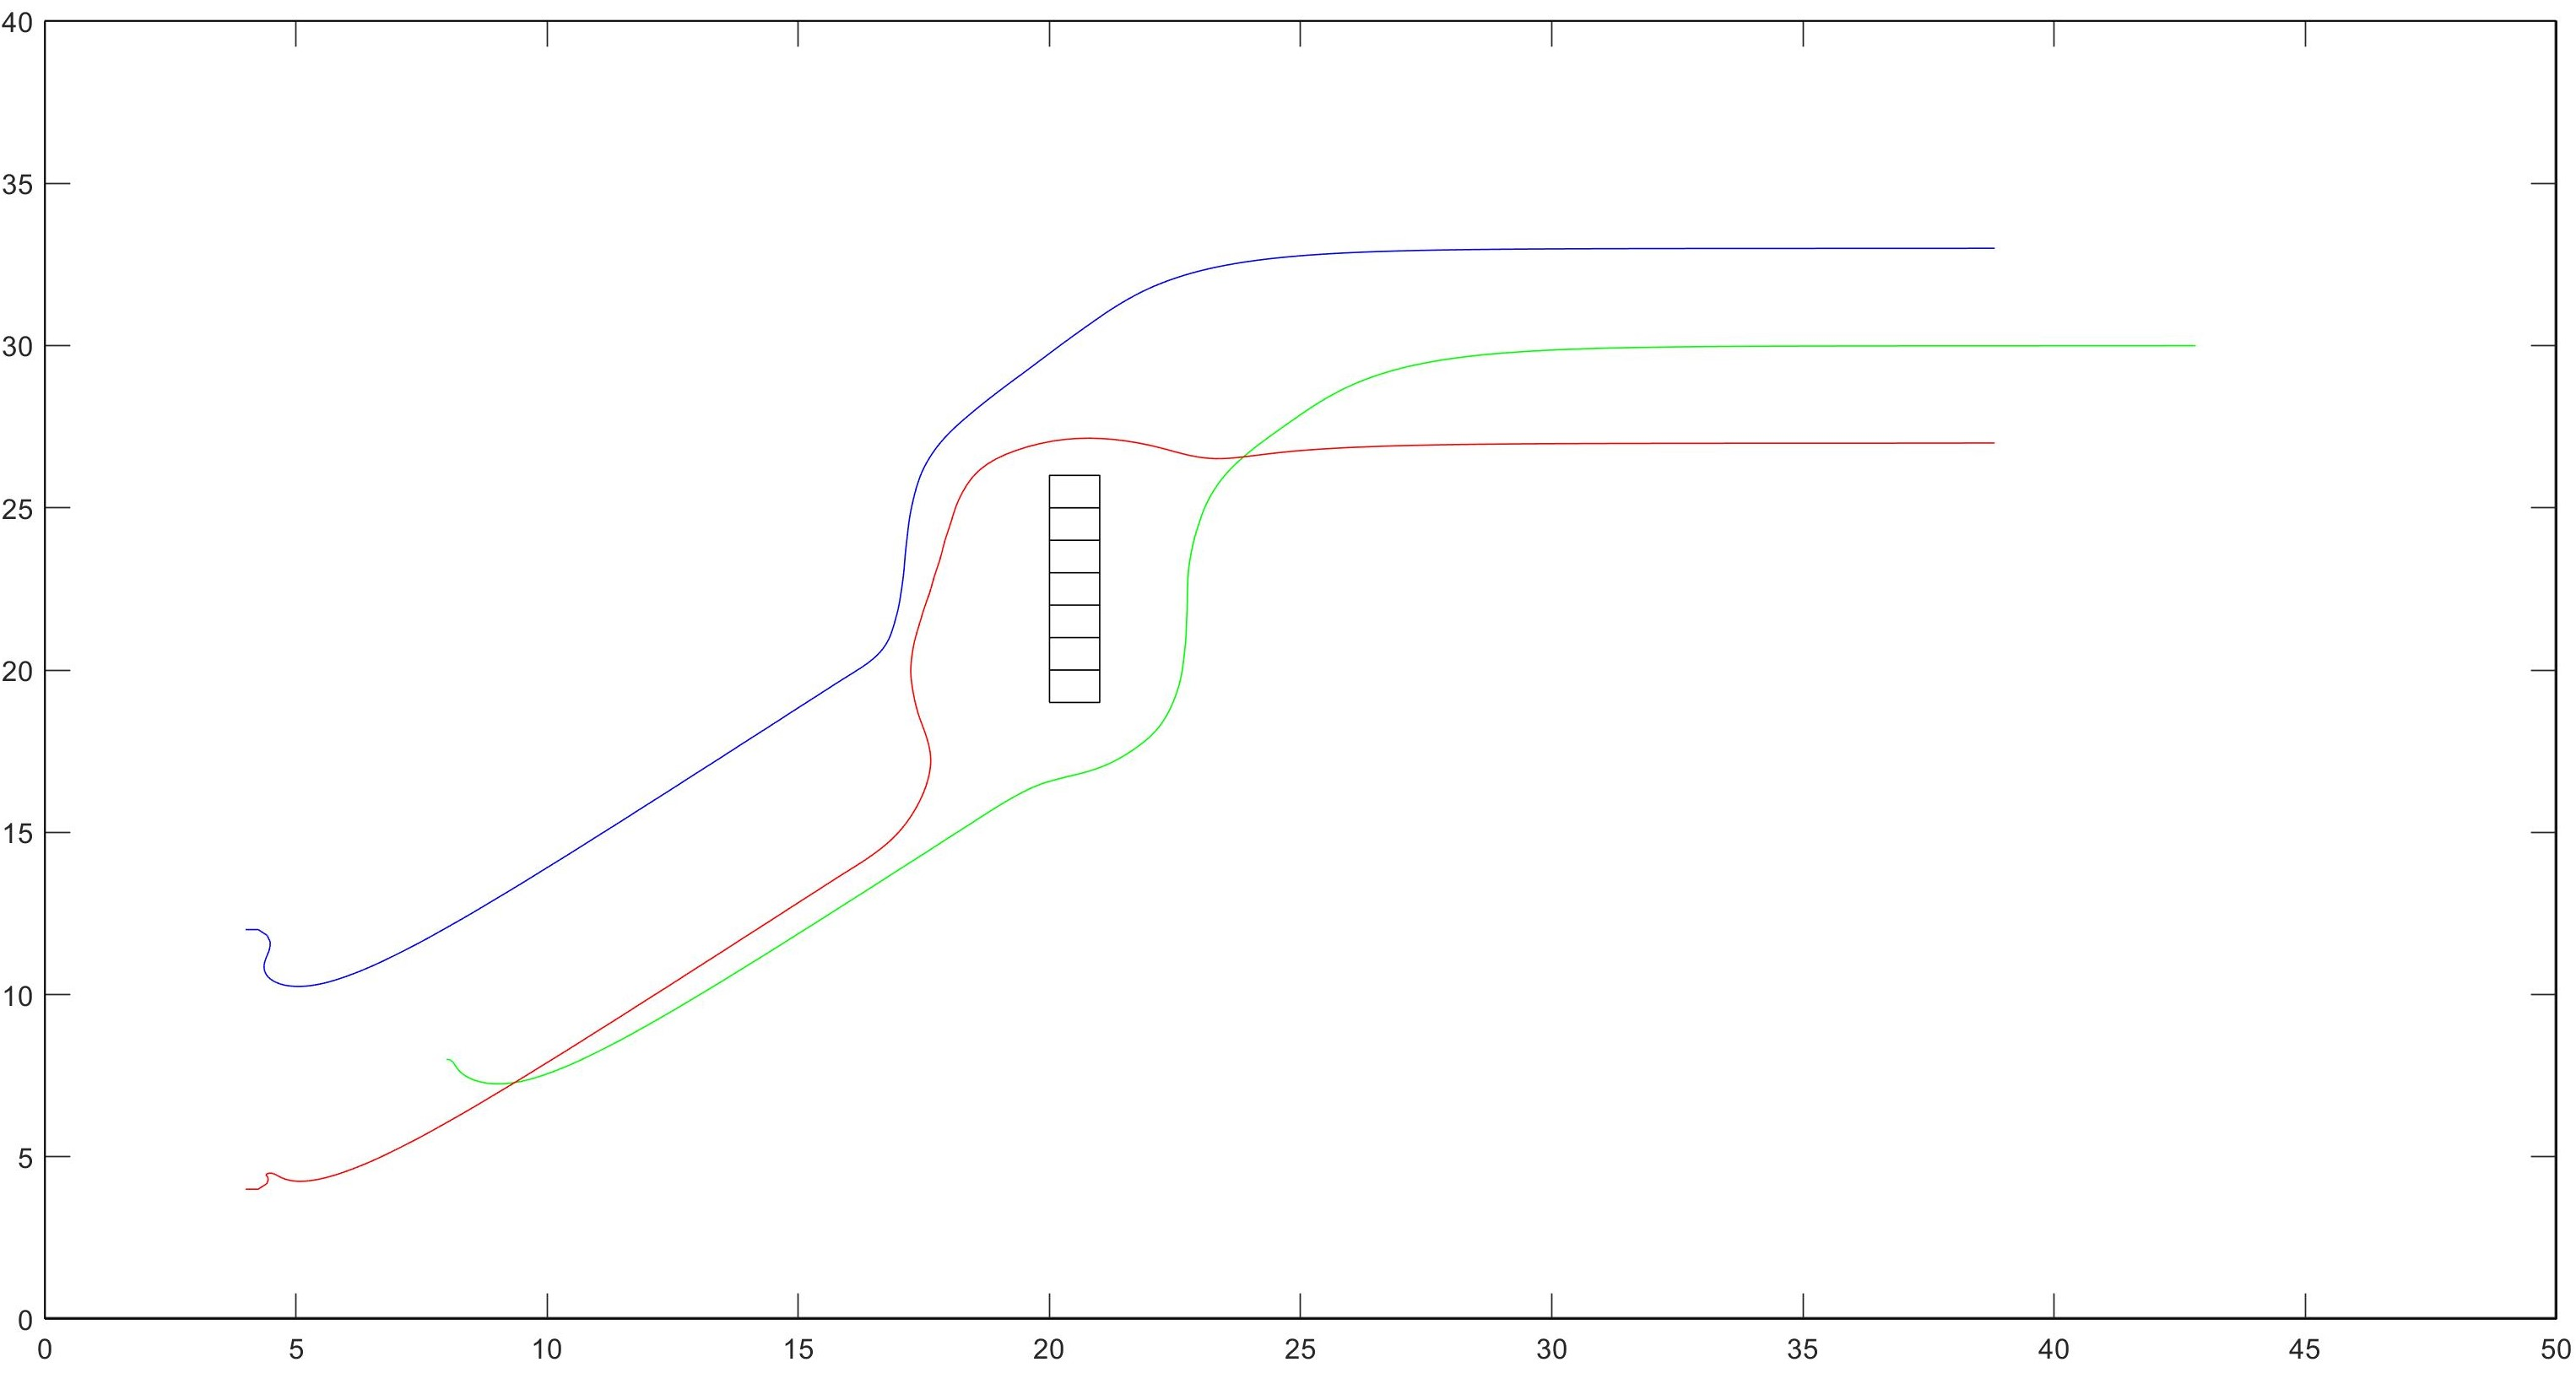
\includegraphics[scale=0.2]{Images/platoon-Greedy-pos.jpg}
	\caption{مکان ربات‌ها در روش $Greedy~best-first~search$}\label{Fig platoon-Greedy-pos}
\end{figure}


\subsection{$A^*$}
روش $A^*$ برای مسیریابی اجماع ربات‌ها در شکل \ref{Fig platoon-A-star-simulink} پیاده‌سازی شده است. مسیر پیموده شده توسط هر ربات، در شکل \ref{Fig platoon-A-star-pos} قابل مشاهده می‌باشد.
\begin{figure}[!h]
	\centering
	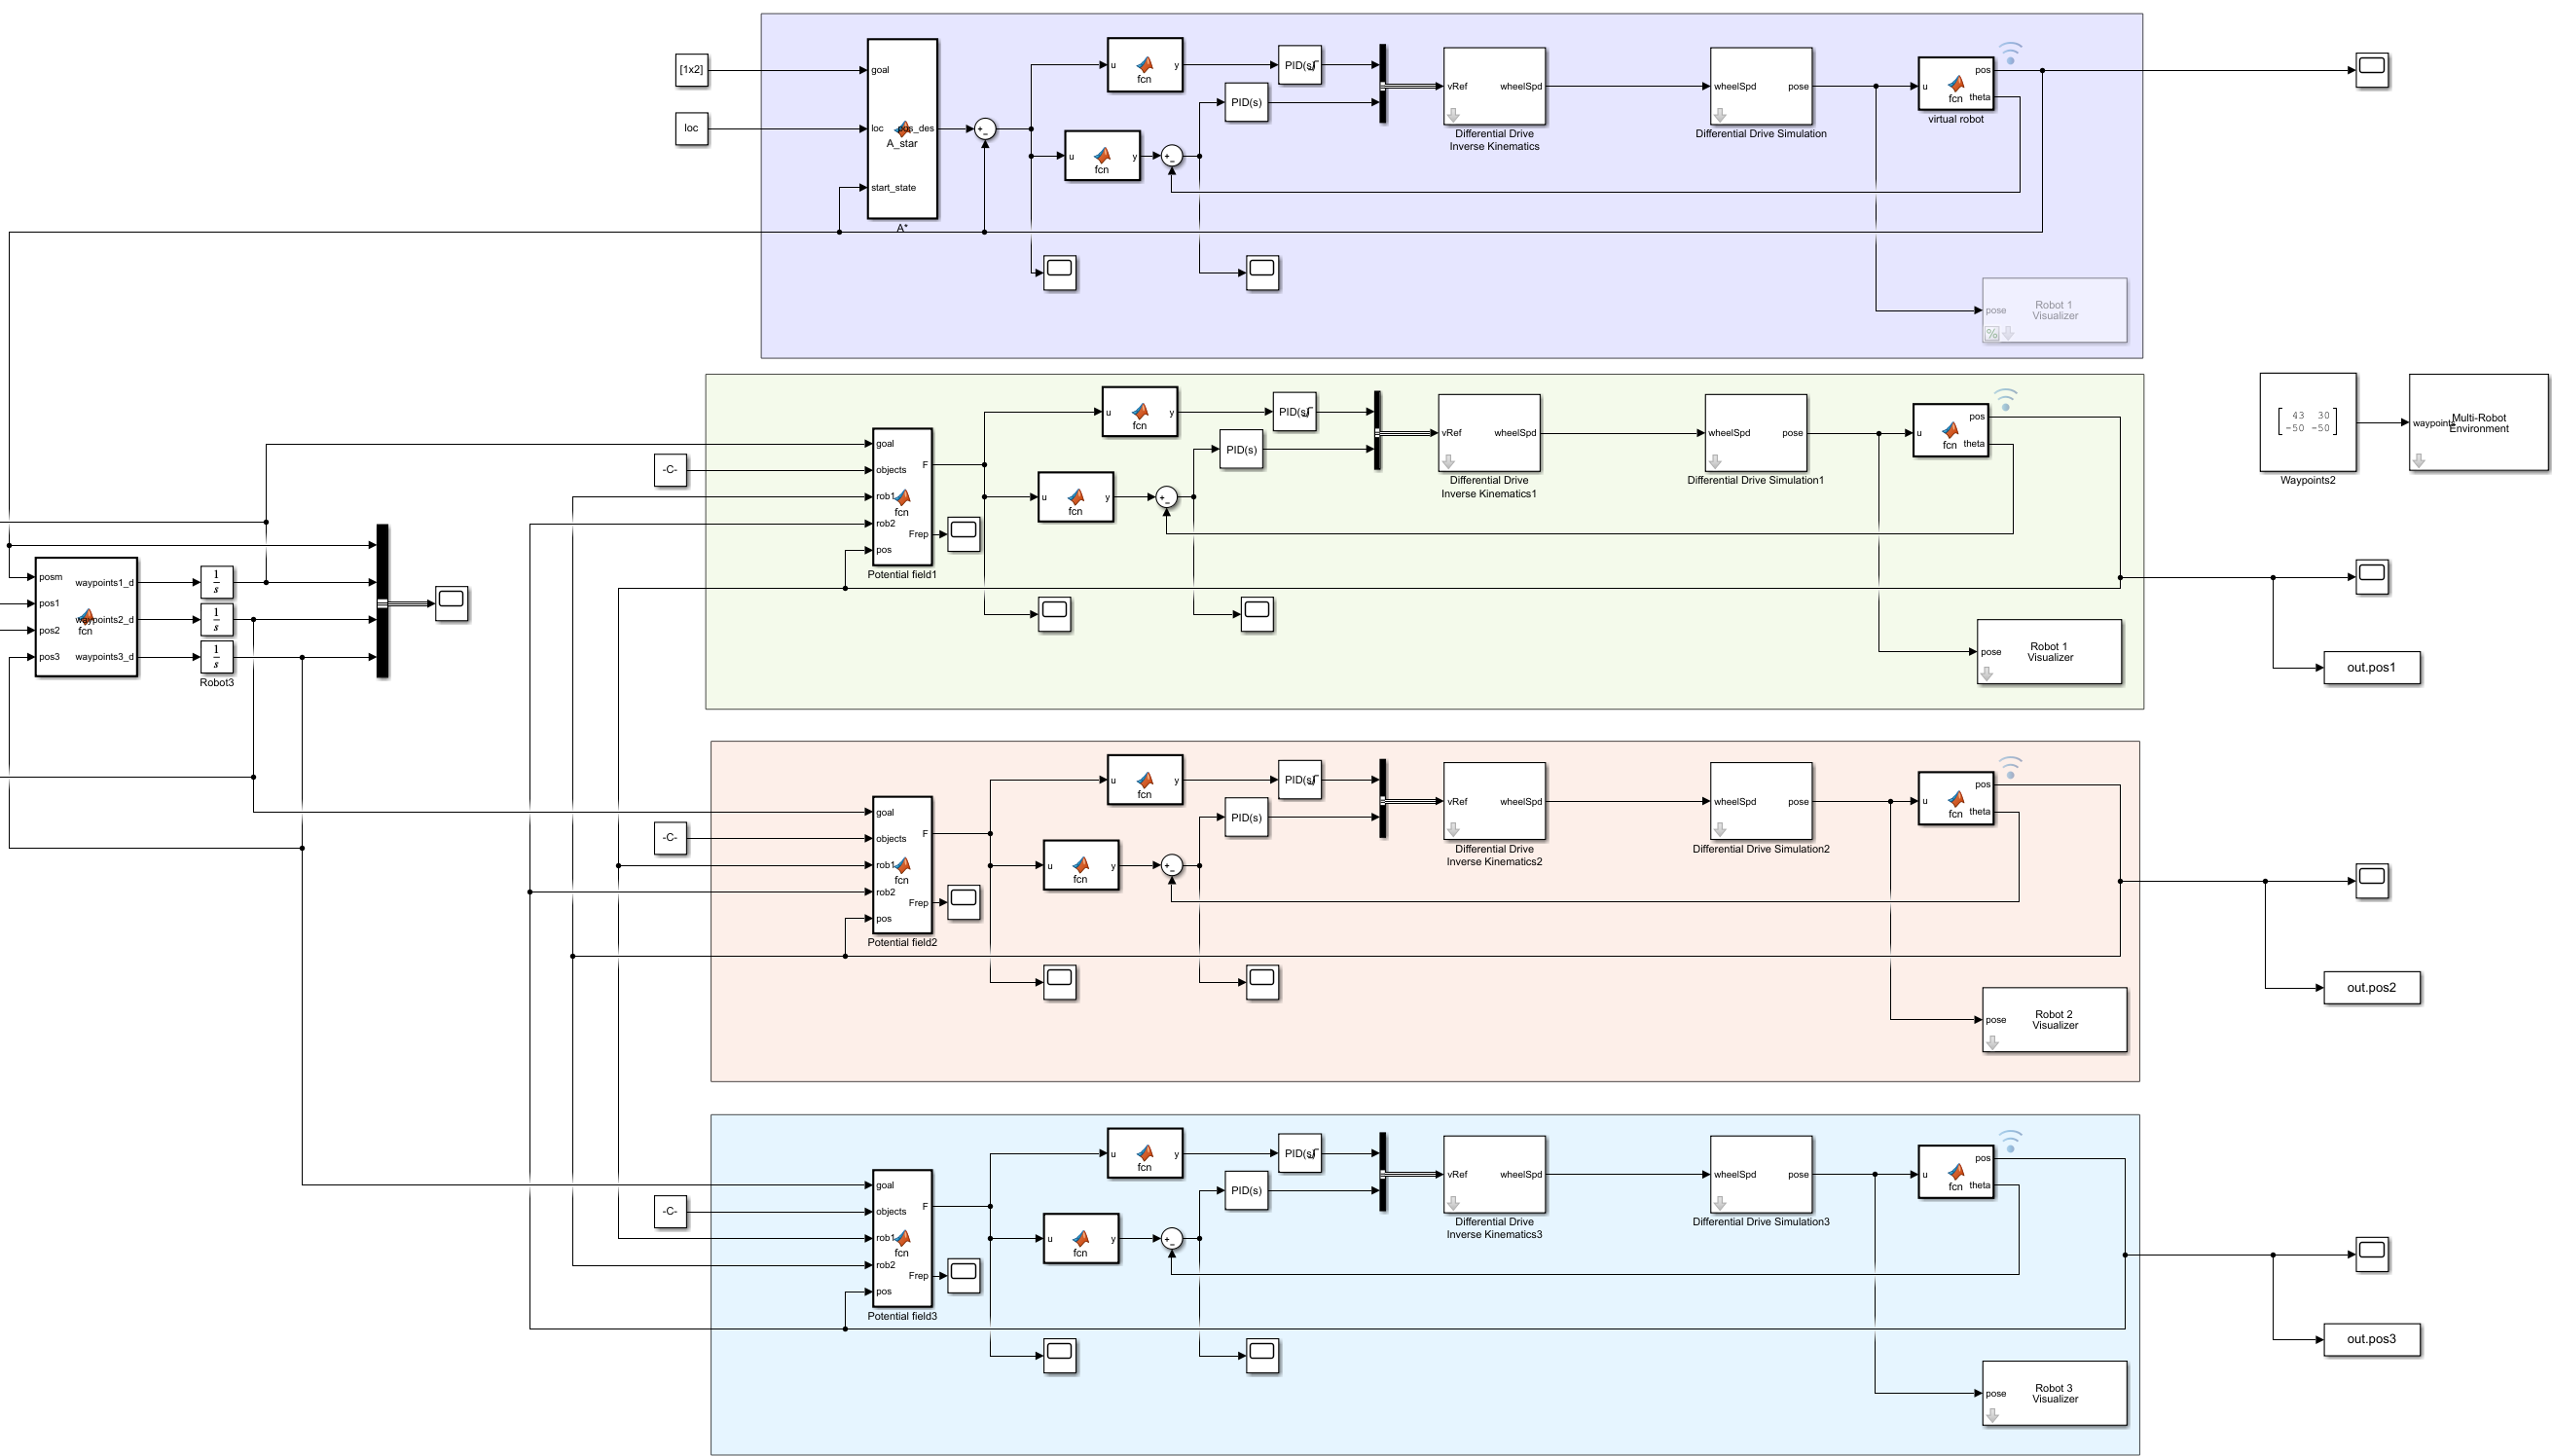
\includegraphics[scale=0.22]{Images/platoon-A-star-simulink.png}
	\caption{بلوک‌های شبیه‌سازی در روش $A^*$}\label{Fig platoon-A-star-simulink}
\end{figure}

\begin{figure}[!h]
	\centering
	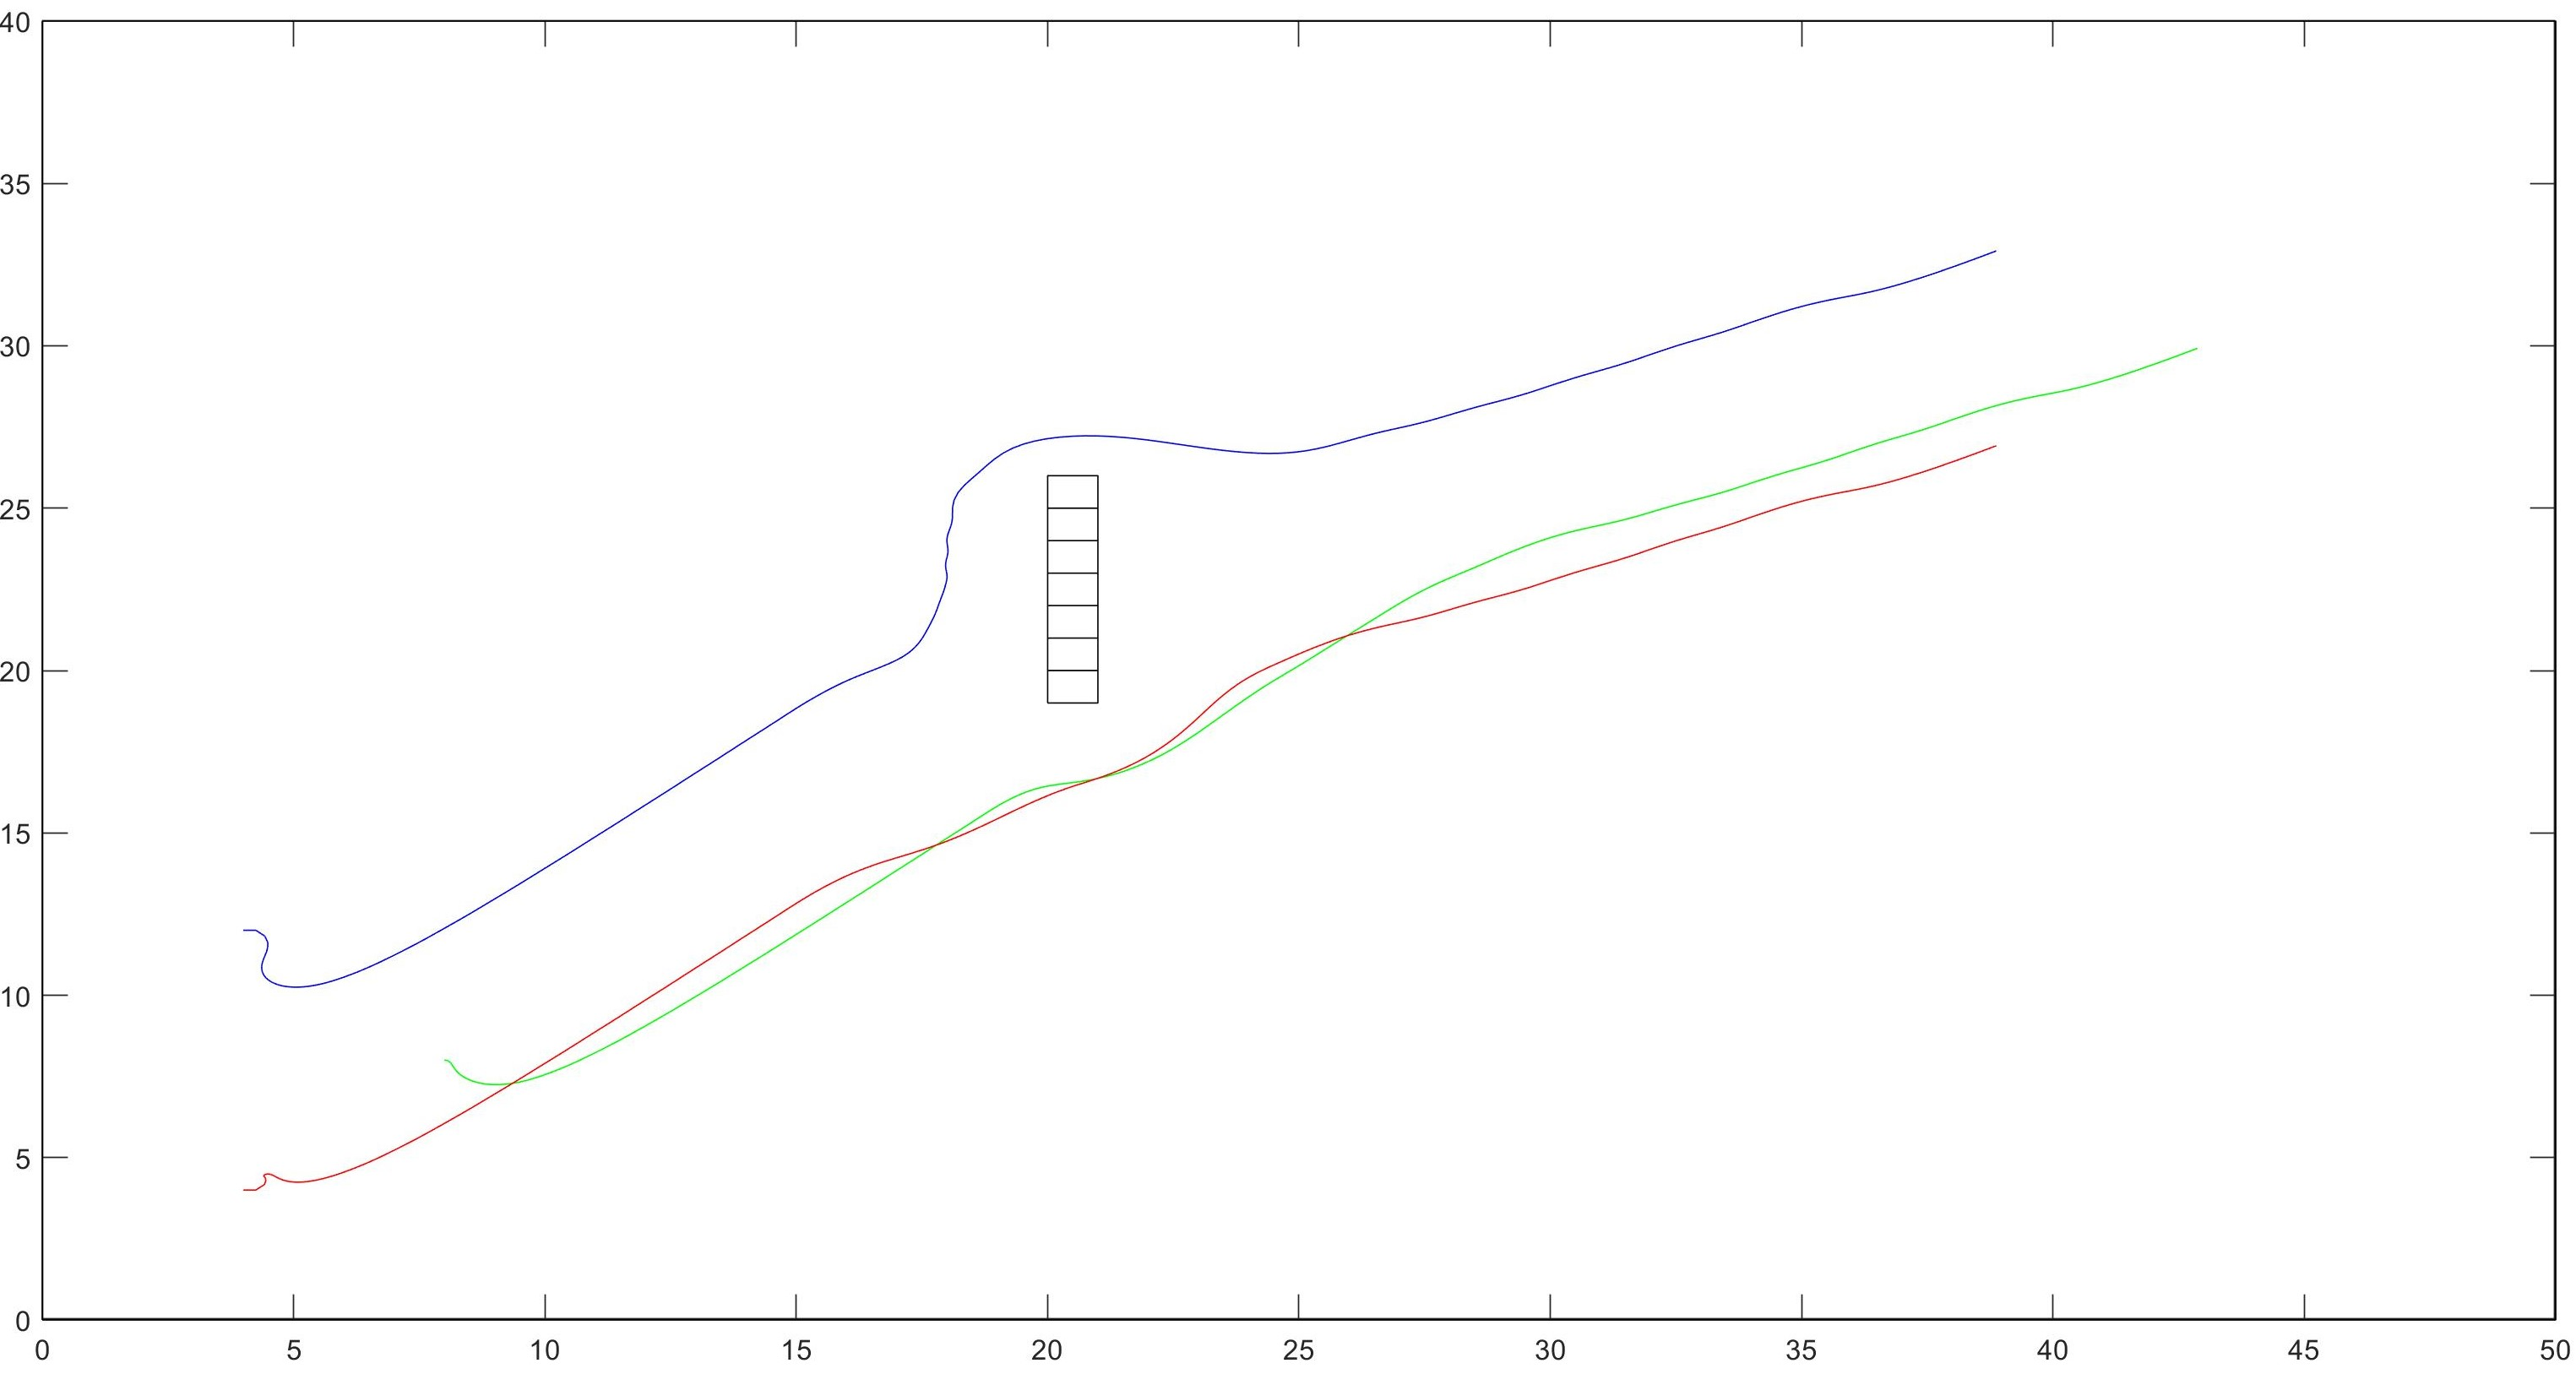
\includegraphics[scale=0.2]{Images/platoon-A-star-pos.jpg}
	\caption{مکان ربات‌ها در روش $A^*$}\label{Fig platoon-A-star-pos}
\end{figure}

\section{$Q-learning$}


















